\documentclass[11pt,a4paper]{article}

% ==============================================================================
% GÓI TIẾNG VIỆT VÀ ĐỊNH DẠNG TRANG IN
% ==============================================================================
\usepackage[utf8]{vietnam}
\usepackage[left=2.2cm,right=2.2cm,top=2cm,bottom=2cm]{geometry}
\usepackage{amsmath,amssymb,amsfonts,amsthm}
\usepackage{graphicx}
\usepackage{booktabs}
\usepackage{tabularx}
\usepackage{multirow}
\usepackage{subcaption}
\usepackage{float}
\usepackage{hyperref}
\usepackage{xcolor}
\usepackage{tikz}
\usetikzlibrary{shapes.geometric, arrows.meta, positioning, calc, shadows}
\usepackage{algorithm}
\usepackage{algpseudocode}
\usepackage{enumitem}
\usepackage{titlesec}
\usepackage{cite}

% Cấu hình liên kết hyperref
\hypersetup{
    colorlinks=true,
    linkcolor=blue!80!black,
    citecolor=red!70!black,
    urlcolor=teal
}

% Cấu hình đường dẫn thư mục ảnh
\graphicspath{{figures/}{./}}

% Cấu hình hiển thị mã giả (Algorithm)
\renewcommand{\algorithmicrequire}{\textbf{Đầu vào:}}
\renewcommand{\algorithmicensure}{\textbf{Đầu ra:}}
\floatname{algorithm}{Thuật toán}

% Định dạng tiêu đề mục chuẩn mực, thoáng đãng
\titleformat{\section}{\large\bfseries\color{blue!80!black}}{\thesection}{1em}{}
\titleformat{\subsection}{\normalsize\bfseries\color{black}}{\thesubsection}{0.8em}{}
\titleformat{\subsubsection}{\small\bfseries\color{black!80!white}}{\thesubsubsection}{0.6em}{}

\usepackage{tcolorbox} 
% ==============================================================================
% PHẦN THÂN TÀI LIỆU
% ==============================================================================
\begin{document}

% ------------------------------------------------------------------------------
% TRANG TIÊU ĐỀ & THÔNG TIN ĐỒ ÁN (TRANG BÌA CÓ KHUNG VÀ LOGO)
% ------------------------------------------------------------------------------
\begin{titlepage}
\begin{tikzpicture}[remember picture,overlay,inner sep=0,outer sep=0]
     \draw[blue!70!black,line width=3.5pt] ([xshift=-1.5cm,yshift=-2cm]current page.north east) coordinate (A)--([xshift=1.5cm,yshift=-2cm]current page.north west) coordinate(B)--([xshift=1.5cm,yshift=2cm]current page.south west) coordinate (C)--([xshift=-1.5cm,yshift=2cm]current page.south east) coordinate(D)--cycle;

     \draw ([yshift=0.4cm,xshift=-0.4cm]A)-- ([yshift=0.4cm,xshift=0.4cm]B)--
     ([yshift=-0.4cm,xshift=0.4cm]B) --([yshift=-0.4cm,xshift=-0.4cm]B)--([yshift=0.4cm,xshift=-0.4cm]C)--([yshift=0.4cm,xshift=0.4cm]C)--([yshift=-0.4cm,xshift=0.4cm]C)-- ([yshift=-0.4cm,xshift=-0.4cm]D)--([yshift=0.4cm,xshift=-0.4cm]D)--([yshift=0.4cm,xshift=0.4cm]D)--([yshift=-0.4cm,xshift=0.4cm]A)--([yshift=-0.4cm,xshift=-0.4cm]A)--([yshift=0.4cm,xshift=-0.4cm]A);

     \draw ([yshift=-0.25cm,xshift=0.25cm]A)-- ([yshift=-0.25cm,xshift=-0.25cm]B)--
     ([yshift=0.25cm,xshift=-0.25cm]B) --([yshift=0.25cm,xshift=0.25cm]B)--([yshift=-0.25cm,xshift=0.25cm]C)--([yshift=-0.25cm,xshift=-0.25cm]C)--([yshift=0.25cm,xshift=-0.25cm]C)-- ([yshift=0.25cm,xshift=0.25cm]D)--([yshift=-0.25cm,xshift=0.25cm]D)--([yshift=-0.25cm,xshift=-0.25cm]D)--([yshift=0.25cm,xshift=-0.25cm]A)--([yshift=0.25cm,xshift=0.25cm]A)--([yshift=-0.25cm,xshift=0.25cm]A);
\end{tikzpicture}

\begin{center}
    \vspace{5pt}
    \textbf{\fontsize{13pt}{15pt}\selectfont TRƯỜNG ĐẠI HỌC KHOA HỌC TỰ NHIÊN, ĐHQG-HCM}
    
    \vspace{4pt}
    \textbf{\fontsize{13pt}{15pt}\selectfont KHOA TOÁN - TIN HỌC}
\end{center}

\vspace{15pt}
\begin{center}
    
\includegraphics[width=0.38\textwidth]{Logo_TA_Doc.png}
    
    \vspace{18pt}
    {\fontsize{15pt}{18pt}\selectfont \textbf{BÁO CÁO ĐỒ ÁN MÔN HỌC}}
    
    \vspace{6pt}
    {\fontsize{16pt}{20pt}\selectfont \textbf{NHẬN DẠNG MẪU (PATTERN RECOGNITION)}}
\end{center}

\vspace{15pt}
\begin{center}
    {\fontsize{12pt}{15pt}\selectfont \textbf{\textsl{ĐỀ TÀI:}}}
    
    \vspace{8pt}
    {\fontsize{15pt}{19pt}\selectfont \textbf{\color{blue!80!black} CÀI ĐẶT VÀ SO SÁNH CÁC MÔ HÌNH HỌC MÁY TRÊN TẬP DỮ LIỆU CHỮ SỐ VIẾT TAY MNIST}}
\end{center}

\vspace{20pt}
\begin{flushleft}
    \fontsize{12pt}{16pt}\selectfont
    \hspace{1.5cm}\textbf{Giảng viên hướng dẫn:} \begin{tabular}[t]{@{}l@{}}
        TS. Trương Phước Hưng \\
        CN. Lê Phú Trường
    \end{tabular}
    
    \vspace{8pt}
    \hspace{1.5cm}\textbf{Sinh viên thực hiện:} \begin{tabular}[t]{@{}l l l@{}}
        1. & Trần Nguyên Hưng & -- MSSV: 24280048 \\
        2. & Vương Thành Đạt  & -- MSSV: 24280058 \\
        3. & Phạm Phương Thảo & -- MSSV: 24280106
    \end{tabular}
\end{flushleft}
\vfill
\begin{center}
    \textbf{\fontsize{11pt}{14pt}\selectfont TP. HỒ CHÍ MINH, THÁNG 11 NĂM 2026}
\end{center}
\vspace{10pt}
\end{titlepage}


\tableofcontents
\newpage

% ==============================================================================
% CHƯƠNG 1: GIỚI THIỆU BÀI TOÁN & QUY TRÌNH TỔNG THỂ (PIPELINE)
% ==============================================================================
\section{Giới thiệu bài toán và Hệ thống}

\subsection{Đặt vấn đề và Mục tiêu}
Bài toán nhận dạng chữ số viết tay trong đồ án này được thực nghiệm trên tập dữ liệu chuẩn MNIST. Bộ dữ liệu gồm 70.000 ảnh xám kích thước $28 \times 28$ pixel (10 nhãn từ 0 đến 9, cường độ $[0, 255]$), chia sẵn thành 60.000 mẫu huấn luyện và 10.000 mẫu kiểm thử. Đồ án tập trung giải quyết ba mục tiêu chính:
\begin{enumerate}[noitemsep]
    \item \textbf{Tiền xử lý dữ liệu:} Phân chia tập huấn luyện thành 50.000 mẫu train và 10.000 mẫu validation theo phương pháp phân tầng (stratified split), đồng thời chuẩn hóa đặc trưng phù hợp từng mô hình.
    \item \textbf{Cài đặt mô hình:} Thực nghiệm 4 mô hình máy học:
    \begin{itemize}[noitemsep]
        \item Mô hình sinh xác suất: Multinomial Naïve Bayes.
        \item Mô hình tuyến tính: One-vs-Rest Logistic Regression.
        \item Mạng nơ-ron: Multi-Layer Perceptron (MLP) và Convolutional Neural Network (CNN).
        \item Học quần thể (Ensemble): AdaBoost kết hợp bộ phân loại yếu.
    \end{itemize}
    \item \textbf{Đánh giá và so sánh:} Đo đạc hiệu năng qua Accuracy, F1-score, ma trận nhầm lẫn cùng thời gian huấn luyện và suy luận để đối sánh ưu nhược điểm giữa các phương pháp.
\end{enumerate}

\subsection{Kiến trúc luồng xử lý (Pipeline)}
Quy trình thực nghiệm của nhóm được minh họa trực quan qua hình sau:

\begin{figure}[H]
\centering
\begin{tikzpicture}[
    data_blk/.style={rectangle, draw=blue!75!black, fill=blue!5, rounded corners=4pt, text width=3.6cm, minimum height=1.2cm, align=center, font=\scriptsize},
    prep_blk/.style={rectangle, draw=teal!80!black, fill=teal!5, rounded corners=4pt, text width=4.3cm, minimum height=1.2cm, align=center, font=\scriptsize},
    model_blk/.style={rectangle, draw=purple!80!black, fill=purple!5, rounded corners=4pt, text width=3.35cm, minimum height=2.2cm, align=center, font=\scriptsize, inner sep=4pt},
    eval_blk/.style={rectangle, draw=orange!85!black, fill=orange!5, rounded corners=4pt, text width=15.4cm, minimum height=1.3cm, align=center, font=\scriptsize, inner sep=4pt},
    arrow/.style={-{Stealth[scale=0.9]}, thick, draw=gray!75!black},
    dist_line/.style={thick, draw=gray!75!black}
]
    % --- HÀNG 1: DỮ LIỆU & TIỀN XỬ LÝ (y = 0) ---
    \node[data_blk] (raw) at (-5.5, 0) {\textbf{\footnotesize Dữ liệu MNIST Gốc}\\70.000 ảnh xám ($28 \times 28$)\\10 chữ số (từ 0 đến 9)};
    \node[prep_blk] (split) at (0, 0) {\textbf{\footnotesize Phân chia dữ liệu}\\Tập Train (50k) / Val (10k)\\Tập Test độc lập (10k)};
    \node[prep_blk] (prep) at (5.5, 0) {\textbf{\footnotesize Tiền xử lý dữ liệu}\\Chuẩn hóa Min-Max $[0, 1]$\\Chuẩn hóa Z-Score};

    \draw[arrow] (raw) -- (split);
    \draw[arrow] (split) -- (prep);

    % --- THANH PHÂN PHỐI DỮ LIỆU (y = -1.15) ---
    \draw[dist_line] (prep.south) -- (5.5, -1.15);
    \draw[dist_line] (-5.7, -1.15) -- (5.7, -1.15);

    % --- HÀNG 2: 4 HƯỚNG MÔ HÌNH (y = -3.0) ---
    \node[model_blk] (bayes) at (-5.7, -3.0) {
        \textbf{\footnotesize Mô hình sinh xác suất}\\[3pt]
        Multinomial Naïve Bayes\\[2pt]
        Làm mượt Laplace ($\alpha^* = 10^{-4}$)\\[2pt]
        Quy tắc hậu nghiệm MAP
    };
    
    \node[model_blk] (logistic) at (-1.9, -3.0) {
        \textbf{\footnotesize Mô hình tuyến tính}\\[3pt]
        One-vs-Rest Logistic Reg.\\[2pt]
        Tốc độ học $\eta^* = 0.5$, $L_2$\\[2pt]
        Vector hóa ma trận trọng số
    };
    
    \node[model_blk] (neural) at (1.9, -3.0) {
        \textbf{\footnotesize Mạng nơ-ron \& Học sâu}\\[3pt]
        MLP (2 tầng ẩn, ReLU, Dropout)\\[2pt]
        CNN (Conv2D, MaxPool, FC)\\[2pt]
        SGD-M \& Adam
    };
    
    \node[model_blk] (rf) at (5.7, -3.0) {
        \textbf{\footnotesize Mô hình học quần thể}\\[3pt]
        AdaBoost Ensemble\\[2pt]
        Cây quyết định nông (Stump)\\[2pt]
        Cập nhật trọng số mẫu
    };

    % Mũi tên từ thanh bus xuống nóc các mô hình
    \draw[arrow] (-5.7, -1.15) -- (bayes.north);
    \draw[arrow] (-1.9, -1.15) -- (logistic.north);
    \draw[arrow] (1.9, -1.15) -- (neural.north);
    \draw[arrow] (5.7, -1.15) -- (rf.north);

    % --- HÀNG 3: ĐÁNH GIÁ TOÀN DIỆN (y = -5.45) ---
    \node[eval_blk] (eval_box) at (0, -5.45) {
        \textbf{\footnotesize Đánh giá toàn diện, So sánh đối chuẩn \& Phân tích lỗi sai}\\[3pt]
        3 tập độc lập (Train, Validation, Test) $\;\bullet\;$ Accuracy, Precision, Recall, Macro-F1, Cross-Entropy Loss\\
        Ma trận nhầm lẫn $\;\bullet\;$ Đánh đổi Độ chính xác -- Tốc độ $\;\bullet\;$ Biểu đồ Radar đa tiêu chí
    };

    % Mũi tên từ đáy các mô hình xuống hộp đánh giá
    \draw[arrow] (bayes.south) -- ([xshift=-5.7cm]eval_box.north);
    \draw[arrow] (logistic.south) -- ([xshift=-1.9cm]eval_box.north);
    \draw[arrow] (neural.south) -- ([xshift=1.9cm]eval_box.north);
    \draw[arrow] (rf.south) -- ([xshift=5.7cm]eval_box.north);
\end{tikzpicture}
\caption{Quy trình tổng thể phân lớp chữ số viết tay MNIST qua 4 mô hình.}
\label{fig:pipeline}
\end{figure}

% ==============================================================================
% CHƯƠNG 2: DỮ LIỆU VÀ TIỀN XỬ LÝ
% ==============================================================================
\section{Khám phá và Tiền xử lý dữ liệu}

\subsection{Phân tích khám phá dữ liệu (EDA)}

Trong bước phân tích khám phá dữ liệu (EDA), nhóm tiến hành thống kê phân phối của 60.000 mẫu huấn luyện và 10.000 mẫu kiểm thử gốc. 

Để phục vụ việc đánh giá và tinh chỉnh mô hình mà không làm rò rỉ dữ liệu kiểm thử, tập huấn luyện được chia tách thành hai tập con: Train (50.000 mẫu) và Validation (10.000 mẫu). Quá trình phân chia được kiểm soát nhằm bảo toàn tỷ lệ xuất hiện đồng đều của 10 lớp chữ số trên cả hai tập, đồng thời đảm bảo khả năng tái lập kết quả thực nghiệm.

\begin{figure}[H]
    \centering
    \begin{subfigure}[b]{0.48\textwidth}
        \centering
        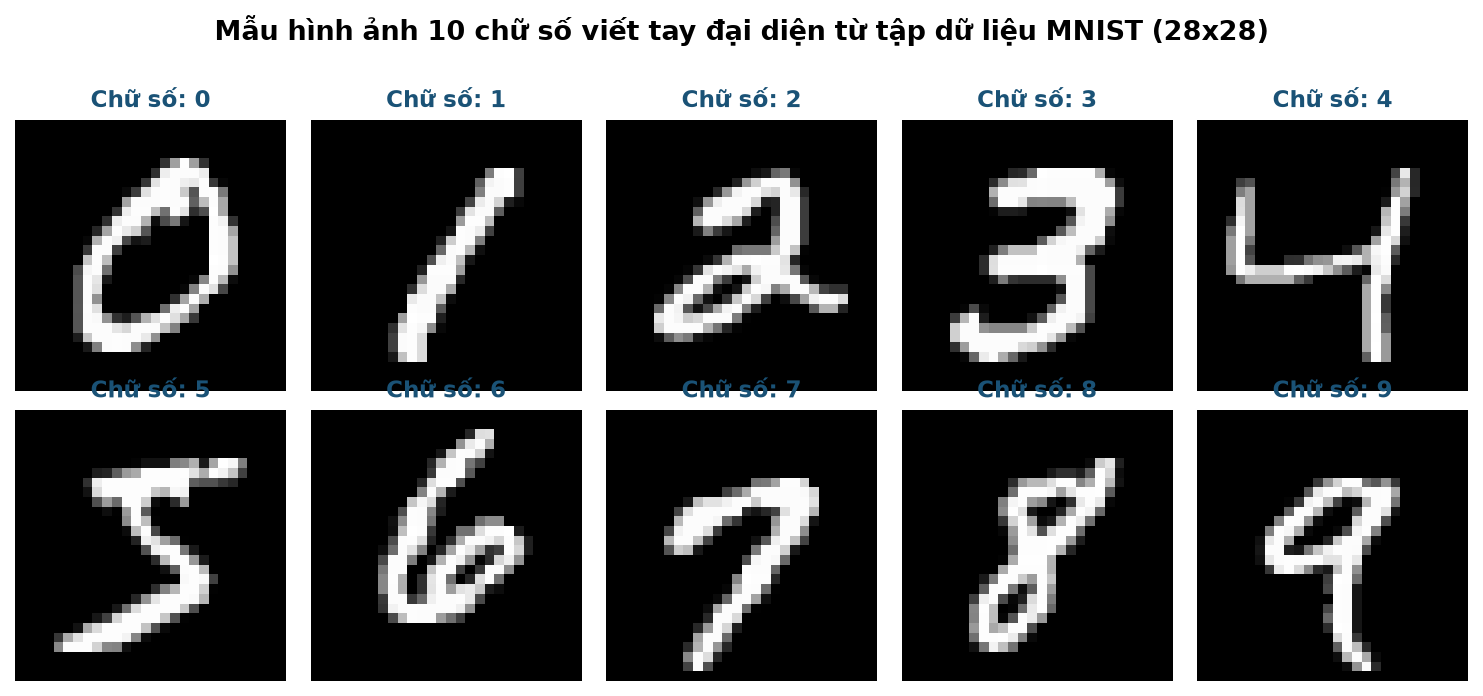
\includegraphics[width=\textwidth]{0_01_sample_digits.png}
        \caption{Mẫu ngẫu nhiên 10 chữ số từ 0 đến 9.}
        \label{fig:sample_digits}
    \end{subfigure}
    \hfill
    \begin{subfigure}[b]{0.48\textwidth}
        \centering
        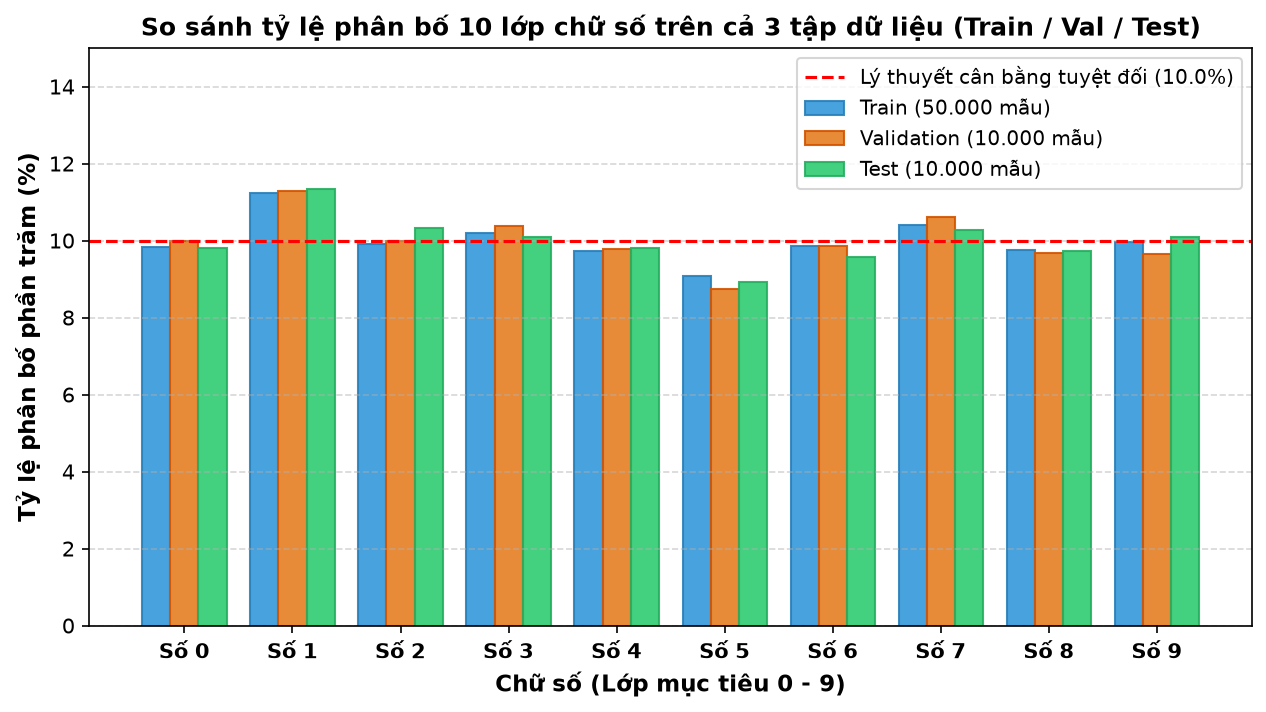
\includegraphics[width=\textwidth]{0_02_class_distribution.png}
        \caption{Phân bố tỷ lệ 10 lớp trên Train/Val/Test.}
        \label{fig:class_dist}
    \end{subfigure}
    \caption{Trực quan hoá dữ liệu khám phá ban đầu trên tập dữ liệu MNIST.}
    \label{fig:eda_plots}
\end{figure}
Từ biểu đồ ở Hình~\ref{fig:eda_plots}, phân phối giữa các chữ số khá đồng đều, dao động từ $8.92\%$ (số 5) đến $11.35\%$ (số 1), cho thấy dữ liệu không bị mất cân bằng lớp. Bên cạnh đó, quá trình kiểm tra và thực nghiệm trên tập dữ liệu ghi nhận thêm hai đặc điểm:
\begin{itemize}[noitemsep]
    \item \textbf{Chất lượng dữ liệu:} Toàn bộ 60.000 mẫu không có giá trị khuyết thiếu (\texttt{NaN}) hay trường hợp trùng lặp.
    \item \textbf{Đặc trưng điểm ảnh:} Có $67/784$ pixel nằm sát 4 cạnh viền luôn bằng $0$ trên mọi mẫu (chiếm $8.55\%$ diện tích), hầu như không mang giá trị phân loại.
\end{itemize}

\begin{figure}[H]
    \centering
    \begin{subfigure}[b]{0.48\textwidth}
        \centering
        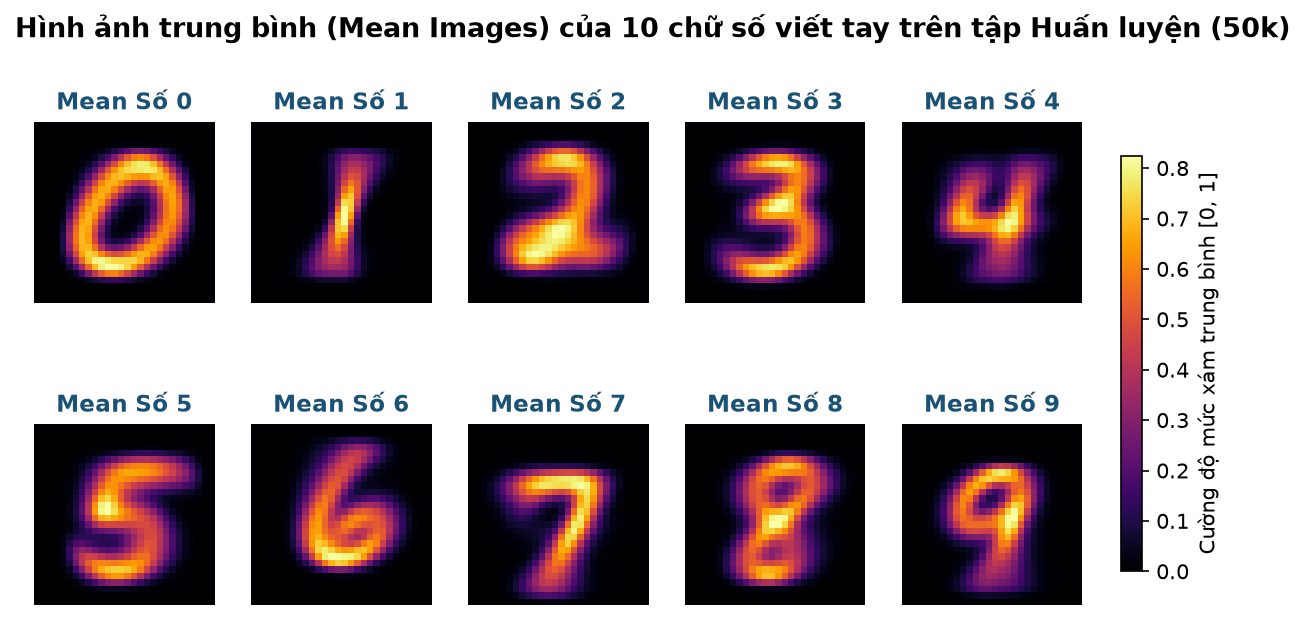
\includegraphics[width=\textwidth]{0_03_mean_digits.png}
        \caption{Ảnh trung bình (Mean Images) của 10 chữ số.}
        \label{fig:mean_digits}
    \end{subfigure}
    \hfill
    \begin{subfigure}[b]{0.48\textwidth}
        \centering
        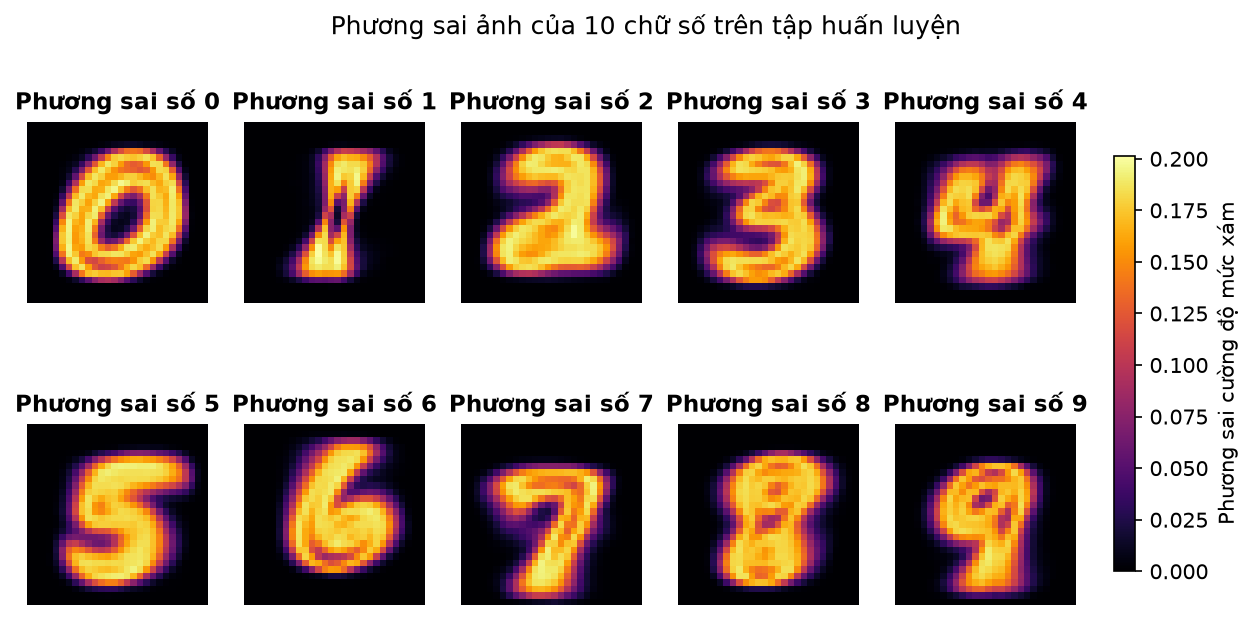
\includegraphics[width=\textwidth]{0_04_variance_digits.png}
        \caption{Phương sai ảnh (Variance Images) của 10 chữ số.}
        \label{fig:var_digits}
    \end{subfigure}
    \caption{Bản đồ nhiệt Ảnh trung bình và Phương sai ảnh của 10 chữ số trên tập Huấn luyện.}
    \label{fig:mean_var_digits}
\end{figure}

\begin{itemize}[noitemsep]
    \item \textbf{Ảnh trung bình (Mean):} Cho thấy hình dạng nét chữ đặc trưng của từng chữ số.
    \item \textbf{Phương sai ảnh (Variance):} Cho thấy mức độ biến thiên về độ nghiêng và nét bút của người viết.
\end{itemize}
Từ đó rút ra hai điểm trọng tâm: một số chữ số có nét tương đồng dễ gây nhầm lẫn (như 4 với 9, hoặc 3, 5 với 8), và 67 pixel viền ngoài có phương sai bằng 0 khiến mô hình Gaussian Naïve Bayes không phù hợp do lỗi chia cho 0.

\subsection{Chuẩn hoá Dữ liệu}

\begin{enumerate}[noitemsep]
    \item \textbf{Chuẩn hoá Min-Max (thang đo $[0, 1]$):} 
    \begin{equation}
        x_{\text{norm}} = \frac{x}{255.0}
    \end{equation}
    Đưa giá trị cường độ điểm ảnh từ khoảng $[0, 255]$ về đoạn $[0, 1]$. Phương pháp này bảo toàn tính không âm ($x \ge 0$), đáp ứng điều kiện đầu vào cho Multinomial Naïve Bayes và giúp giải thuật tối ưu của Logistic Regression hội tụ tốt hơn.

    \item \textbf{Chuẩn hoá Z-score (Standardization):}
    \begin{equation}
        x_{\text{std}} = \frac{x - \mu}{\sigma + \epsilon}
    \end{equation}
    Biến đổi dữ liệu về phân phối có kỳ vọng xấp xỉ 0 và phương sai bằng 1 với $\mu$ và $\sigma$ là giá trị trung bình và độ lệch chuẩn tính trên tập huấn luyện, $\epsilon$ là số thực dương rất nhỏ nhằm tránh lỗi chia cho 0. Cách chuẩn hoá này giúp ổn định biên độ lan truyền và tối ưu hoá gradient cho các mô hình mạng nơ-ron (MLP).
\end{enumerate}

% ==============================================================================
% CHƯƠNG 3: MULTINOMIAL NAIVE BAYES
% ==============================================================================
\section{Mô hình 1: Multinomial Naïve Bayes}

\subsection{Phương pháp và Quy trình xử lý}
Multinomial Naïve Bayes mô hình hóa mỗi bức ảnh như một tập hợp các hạt mực phân bố trên $d = 784$ pixel. Với giả định các pixel độc lập có điều kiện theo từng lớp chữ số, nhãn dự đoán được xác định theo quy tắc hậu nghiệm cực đại (MAP) trong miền Log:
\begin{equation}
    \hat{y} = \arg\max_{c \in \{0, \dots, 9\}} \left[ \ln P(y = c) + \sum_{j=1}^d x_j \ln \theta_{cj} \right]
\end{equation}
Trong đó $P(y = c)$ là xác suất tiên nghiệm của lớp $c$, $\theta_{cj}$ là xác suất hạt mực rơi vào pixel thứ $j$ của chữ số $c$. Số hạng giai thừa trong phân phối đa thức độc lập với $c$ nên triệt tiêu khi lấy $\arg\max$, giúp tránh tràn số và tối ưu tốc độ tính toán.

Do các pixel ở viền ảnh luôn bằng 0, ước lượng xác suất thuần túy sẽ dẫn đến $\theta_{cj} = 0 \implies \ln(0) = -\infty$. Để khắc phục, nhóm áp dụng kỹ thuật làm mượt Laplace với hệ số $\alpha > 0$:
\begin{equation}
    \hat{\theta}_{cj} = \frac{\mu_{cj} + \alpha}{\sum_{k=1}^d \mu_{ck} + d \cdot \alpha}
\end{equation}
với $\mu_{cj}$ là cường độ trung bình của pixel $j$ trong lớp $c$, và mẫu số cộng thêm $d \cdot \alpha$ để bảo toàn điều kiện chuẩn hóa xác suất $\sum_{j=1}^d \hat{\theta}_{cj} = 1$.

\noindent
\textbf{Quy trình xử lý (Pipeline):}
\begin{center}
\begin{tikzpicture}[
    node distance=0.28cm,
    stage/.style={
        rectangle, 
        draw=teal!80!black, 
        fill=teal!5, 
        line width=0.8pt,
        rounded corners=5pt, 
        font=\scriptsize, 
        align=center, 
        inner sep=4pt, 
        text width=3.58cm, 
        minimum height=1.35cm,
        drop shadow={opacity=0.08, shadow xshift=1pt, shadow yshift=-1pt}
    },
    arr/.style={-{Stealth[length=5pt, width=4pt]}, line width=1.1pt, draw=teal!80!black}
]
    \node[stage] (s1) {{\color{teal!90!black}\textbf{1. Thống kê dữ liệu}}\\[2pt]Tính vector kỳ vọng $\boldsymbol{\mu}_c$\\[1pt]và tiên nghiệm $P(y=c)$};
    \node[stage, right=of s1] (s2) {{\color{teal!90!black}\textbf{2. Làm mượt Laplace}}\\[2pt]Ước lượng $\hat{\boldsymbol{\theta}}_c$ với $\alpha^*$\\[1pt]Tránh lỗi $\ln(0) = -\infty$};
    \node[stage, right=of s2] (s3) {{\color{teal!90!black}\textbf{3. Điểm số Log-MAP}}\\[2pt]$\mathbf{S} = \ln \mathbf{P} + \mathbf{X}\ln\boldsymbol{\Theta}^T$\\[1pt]Triệt tiêu giai thừa};
    \node[stage, right=of s3] (s4) {{\color{teal!90!black}\textbf{4. Dự đoán nhãn}}\\[2pt]$\hat{\mathbf{y}} = \arg\max_{c} \mathbf{S}[:, c]$\\[1pt]Gán nhãn điểm lớn nhất};

    \draw[arr] (s1) -- (s2);
    \draw[arr] (s2) -- (s3);
    \draw[arr] (s3) -- (s4);
\end{tikzpicture}
\end{center}
Thuật toán huấn luyện và suy luận Multinomial Naïve Bayes được mô tả trong Thuật toán~\ref{alg:naive_bayes}.
\begin{algorithm}[H]
\caption{Huấn luyện và Dự đoán Multinomial Naïve Bayes}
\label{alg:naive_bayes}
\begin{algorithmic}[1]
\Require Tập huấn luyện $\mathbf{X} \in [0, 1]^{N \times d}$, nhãn $\mathbf{y} \in \{0, \dots, 9\}^N$, hệ số $\alpha$, tập kiểm thử $\mathbf{X}_{\text{test}}$.
\Ensure Vector nhãn dự đoán $\hat{\mathbf{y}}_{\text{test}}$.
\Statex \textbf{// Giai đoạn huấn luyện (Hàm fit):}
\For{mỗi lớp $c \in \{0, 1, \dots, 9\}$}
    \State Lọc các mẫu thuộc lớp $c$: $\mathbf{X}_c \leftarrow \mathbf{X}[\mathbf{y} == c]$
    \State Xác suất tiên nghiệm: $\text{prior}[c] \leftarrow \frac{|\mathbf{X}_c|}{N}$
    \State Cường độ trung bình từng pixel: $\boldsymbol{\mu}_c \leftarrow \frac{1}{|\mathbf{X}_c|} \sum_{\mathbf{x} \in \mathbf{X}_c} \mathbf{x}$
\EndFor
\Statex \textbf{// Giai đoạn dự đoán (Hàm predict\_log\_proba \& predict):}
\For{mỗi lớp $c \in \{0, 1, \dots, 9\}$}
    \State Xác suất rơi mực Laplace: $\boldsymbol{\theta}_c \leftarrow \frac{\boldsymbol{\mu}_c + \alpha}{\sum_{j=1}^d (\mu_{cj} + \alpha)}$
    \State Log-likelihood của $N_{\text{test}}$ mẫu: $\mathbf{L}_c \leftarrow \sum_{j=1}^d x_{ij} \ln \theta_{cj}$
    \State Điểm số hậu nghiệm: $\mathbf{S}[:, c] \leftarrow \mathbf{L}_c + \ln \text{prior}[c]$
\EndFor
\State Gán nhãn có điểm lớn nhất: $\hat{\mathbf{y}}_{\text{test}} \leftarrow \arg\max_{c \in \{0, \dots, 9\}} \mathbf{S}[:, c]$
\State \Return $\hat{\mathbf{y}}_{\text{test}}$
\end{algorithmic}
\end{algorithm}

\subsection{Thí nghiệm, Đối chiếu Scikit-Learn và Đánh giá Kết quả}
\textbf{Khảo sát siêu tham số làm mượt Laplace $\alpha$:} Nhóm tiến hành khảo sát lưới siêu tham số trên thang đo Logarit $\alpha \in [10^{-6}, 10^{-5}, 10^{-4}, 10^{-3}, 10^{-2}, 0.1, 1.0, 10.0, 100.0]$ trên tập Validation ($10.000$ mẫu). Kết quả trên Hình~\ref{fig:alpha_tuning} cho thấy điểm cực trị đạt được tại $\alpha^* = 10^{-4}$ với độ chính xác cao nhất đạt $82.15\%$ trên tập Validation và $83.56\%$ trên tập Test. Khi tăng $\alpha \ge 1.0$, độ chính xác suy giảm rõ rệt và tụt xuống $62.57\%$ khi $\alpha = 100.0$ do hiện tượng làm mượt quá mức làm san phẳng phân phối đặc trưng (Underfitting).

\begin{figure}[H]
    \centering
    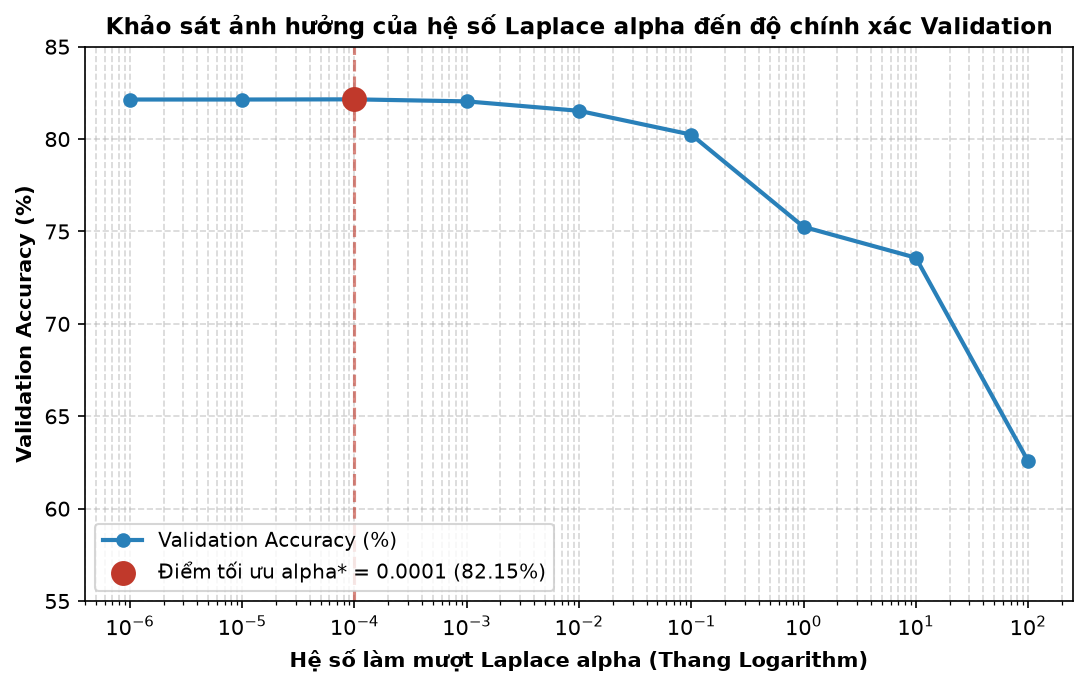
\includegraphics[width=0.68\textwidth]{1_01_laplace_alpha_tuning.png}
    \caption{Khảo sát siêu tham số Laplace smoothing $\alpha$ trên tập Validation (đỉnh tối ưu tại $\alpha^* = 10^{-4}$).}
    \label{fig:alpha_tuning}
\end{figure}

\noindent
\textbf{Đối chiếu Scikit-Learn:} Kiểm chứng trực tiếp với mô hình \texttt{MultinomialNB} của thư viện Scikit-Learn ở cùng giá trị $\alpha^* = 10^{-4}$ cho thấy mô hình tự cài đặt đạt độ chính xác $83.56\%$, bám sát kết quả của thư viện ($83.63\%$, chênh lệch chỉ $0.07\%$) và tỷ lệ đồng thuận dự đoán đạt trên $99.8\%$, khẳng định tính chính xác của thuật toán cài đặt.

\begin{table}[H]
\centering
\small
\caption{Kết quả thực nghiệm của Multinomial Naïve Bayes ($\alpha^* = 10^{-4}$).}
\label{tab:bayes_results}
\resizebox{0.92\textwidth}{!}{%
\begin{tabular}{lrrrrrr}
\toprule
\textbf{Tập dữ liệu} & \textbf{Số mẫu} & \textbf{Accuracy (\%)} & \textbf{Precision (\%)} & \textbf{Recall (\%)} & \textbf{Macro F1 (\%)} & \textbf{Thời gian (s)} \\
\midrule
Train & 50.000 & 82.47 & 83.19 & 82.18 & 82.35 & \textbf{0.06} \\
Validation & 10.000 & 82.15 & 82.77 & 81.80 & 81.98 & \textbf{0.03} \\
Test & 10.000 & \textbf{83.56} & 84.24 & 83.25 & 83.41 & \textbf{0.03} \\
\bottomrule
\end{tabular}%
}
\end{table}

\begin{figure}[H]
    \centering
    \begin{subfigure}[b]{0.48\textwidth}
        \centering
        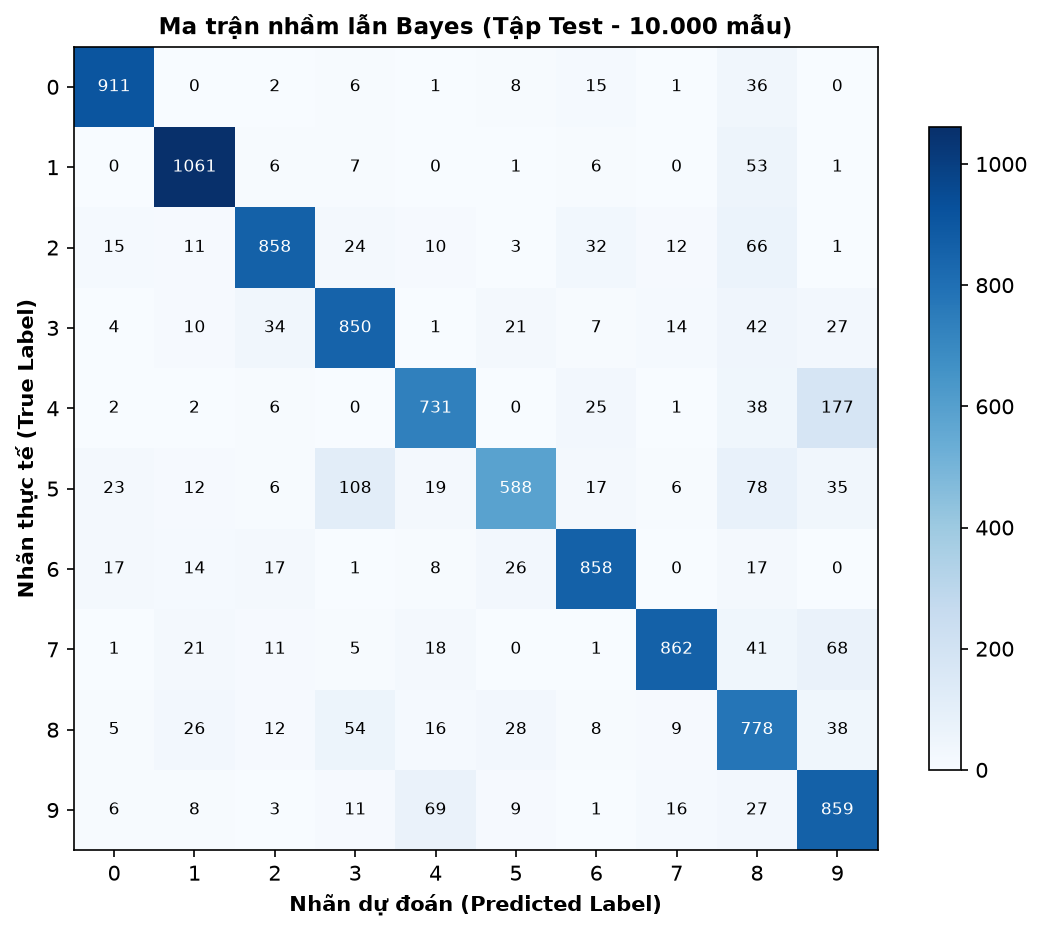
\includegraphics[width=\textwidth]{1_04_bayes_confusion_test.png}
        \caption{MNB - Confushion Test (Accuracy = 83.56\%).}
        \label{fig:bayes_cm}
    \end{subfigure}
    \hfill
    \begin{subfigure}[b]{0.48\textwidth}
        \centering
        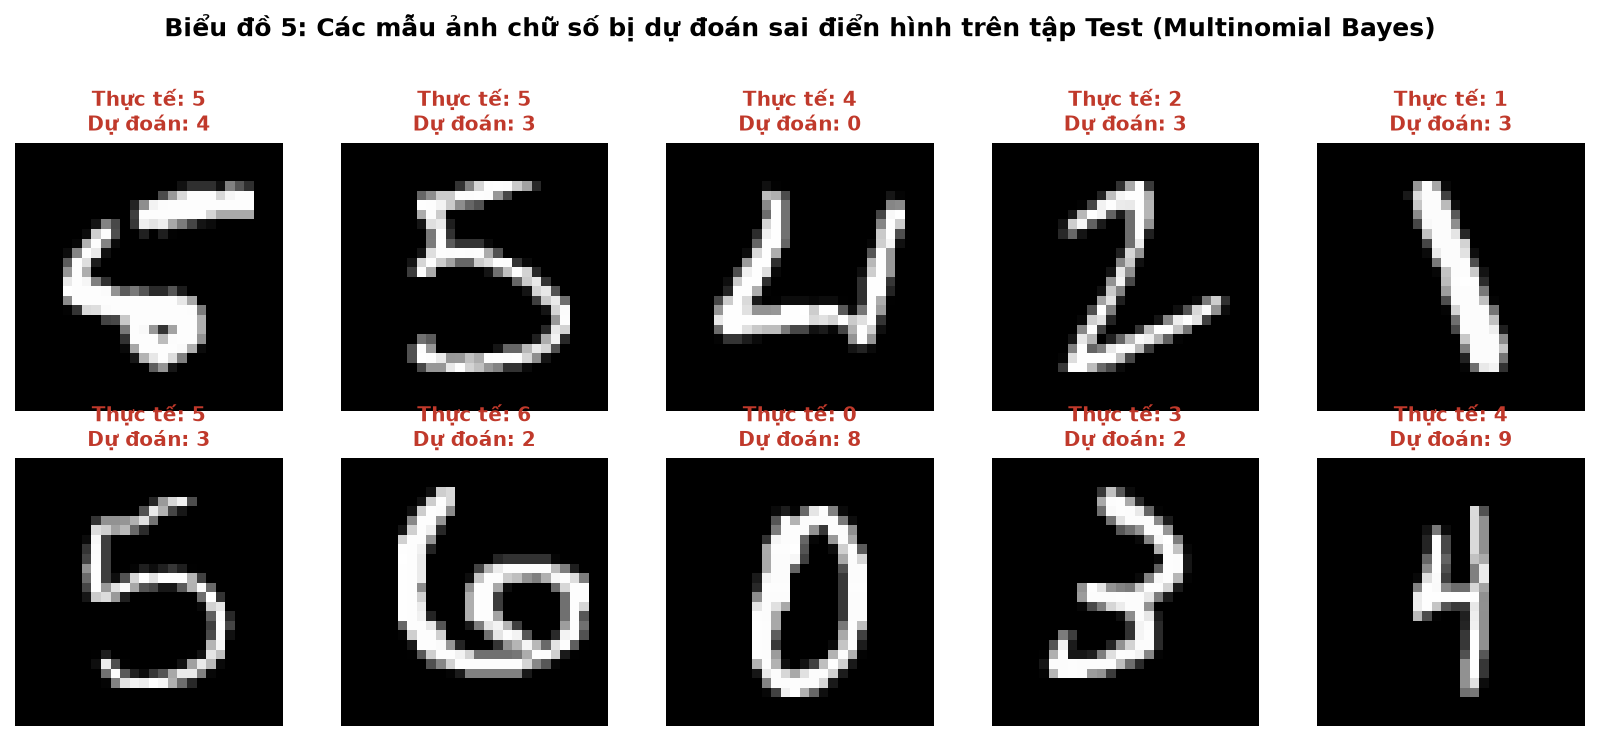
\includegraphics[width=\textwidth]{1_05_bayes_misclassified_samples.png}
        \caption{Các mẫu ảnh bị nhận diện sai điển hình.}
        \label{fig:bayes_errors}
    \end{subfigure}
    \caption{Ma trận nhầm lẫn và các trường hợp lỗi phân loại của Multinomial Naïve Bayes.}
    \label{fig:bayes_cm_errors}
\end{figure}
\noindent
\textbf{Nhận xét kết quả thực nghiệm:}
\begin{itemize}[noitemsep]
    \item \textbf{Hiệu năng tính toán:} Mô hình có tốc độ huấn luyện rất cao ($0.06$ giây cho $50.000$ mẫu) và độ trễ suy luận chỉ khoảng $0.03$ ms/mẫu. Điều này đạt được do thuật toán chỉ thực hiện ước lượng tham số qua đếm tần suất thống kê thay vì tối ưu hóa lặp đi lặp lại.
    \item \textbf{Độ chính xác theo lớp:} Nhận diện tốt nhất ở chữ số 0 ($F_1 = 92.77\%$) và 1 ($F_1 = 92.26\%$) nhờ cấu trúc nét đơn giản, ít trùng lặp. Ngược lại, số 5 có Recall thấp nhất ($65.92\%$, bỏ sót 304 mẫu) và số 8 có Precision thấp nhất ($66.16\%$, có 398 mẫu bị phân loại nhầm thành số 8).
    \item \textbf{Phân tích lỗi và nguyên nhân:} Sự nhầm lẫn chủ yếu ở cặp số (4, 9) và cặp (5 $\to$ 3). Nguyên nhân do giả định độc lập có điều kiện ($x_j \perp x_k \mid y = c$) bỏ qua tương quan không gian giữa các pixel, khiến mô hình chỉ dựa vào phân bố cường độ điểm ảnh riêng lẻ mà không nắm bắt được cấu trúc nét vẽ liền mạch.
\end{itemize}
\section{Mô hình 2: One-vs-Rest Logistic Regression}

\subsection{Phương pháp và Quy trình xử lý}
Logistic Regression là mô hình phân biệt tuyến tính, tối ưu hóa trực tiếp xác suất phân lớp của mẫu dữ liệu. Để giải quyết bài toán nhận dạng 10 chữ số, nhóm áp dụng chiến lược One-vs-Rest, huấn luyện đồng thời 10 bộ phân loại nhị phân tương ứng với 10 lớp ($c \in \{0, \dots, 9\}$).

Với mỗi mẫu ảnh được chèn bias $\tilde{\mathbf{x}} = [\mathbf{x}, 1] \in \mathbb{R}^{785}$ và vector trọng số $\mathbf{w}_c \in \mathbb{R}^{785}$, điểm số tuyến tính $z = \tilde{\mathbf{x}}\mathbf{w}_c$ được chuyển thành xác suất thông qua hàm Sigmoid phân nhánh để chống tràn số:
\begin{equation}
    \sigma(z) = \begin{cases} \dfrac{1}{1 + e^{-z}}, & z \ge 0 \\[6pt] \dfrac{e^z}{1 + e^z}, & z < 0 \end{cases}
\end{equation}
Hàm mất mát Binary Cross-Entropy kết hợp điều chuẩn $L_2$ cho từng chữ số $c$ có dạng:
\begin{equation}
    J(\mathbf{w}_c) = \frac{1}{N}\sum_{i=1}^N \Big[ \ln(1 + e^{z_{ic}}) - t_{ic}z_{ic} \Big] + \frac{\lambda}{2}\|\mathbf{m} \odot \mathbf{w}_c\|^2
\end{equation}
với $z_{ic} = \tilde{\mathbf{x}}_i \mathbf{w}_c$ và $t_{ic} \in \{0, 1\}$ là nhãn One-hot của mẫu $i$ đối với chữ số $c$. Biểu thức $\ln(1 + e^z)$ được tính toán bằng \texttt{np.logaddexp(0, z)} giúp triệt tiêu hoàn toàn nguy cơ tràn số. Vector mặt nạ $\mathbf{m} = [1, \dots, 1, 0]^T \in \mathbb{R}^{785}$ đảm bảo không phạt điều chuẩn lên hệ số tự do $w_0$, giúp các siêu phẳng tự do dịch chuyển tịnh tiến mà không làm méo ranh giới phân lớp.

\noindent
\textbf{Kỹ thuật Vector hóa ma trận:} Thay vì lặp tuần tự 10 bộ phân loại, nhóm gộp toàn bộ tham số thành ma trận trọng số $\mathbf{W} \in \mathbb{R}^{785 \times 10}$ và ma trận nhãn $\mathbf{T} \in \{0, 1\}^{N \times 10}$. Toàn bộ quá trình tính đạo hàm Gradient được thực hiện song song bằng một phép nhân ma trận:
\begin{equation}
    \nabla_{\mathbf{W}} J = \frac{1}{N}\tilde{\mathbf{X}}^T(\mathbf{P} - \mathbf{T}) + \lambda(\mathbf{m} \odot \mathbf{W}), \quad \mathbf{W} \leftarrow \mathbf{W} - \eta \nabla_{\mathbf{W}} J
\end{equation}
Trong đó $\mathbf{P} = \sigma(\tilde{\mathbf{X}}\mathbf{W}) \in [0, 1]^{N \times 10}$ là ma trận xác suất dự đoán, và $\eta$ là tốc độ học.

\noindent
\textbf{Quy trình xử lý:}
\begin{center}
\begin{tikzpicture}[
    node distance=0.25cm,
    stage/.style={
        rectangle, 
        draw=purple!80!black, 
        fill=purple!5, 
        line width=0.8pt,
        rounded corners=5pt, 
        font=\scriptsize, 
        align=center, 
        inner sep=4pt, 
        minimum height=1.35cm,
        drop shadow={opacity=0.08, shadow xshift=1pt, shadow yshift=-1pt}
    },
    arr/.style={-{Stealth[length=5pt, width=4pt]}, line width=1.1pt, draw=purple!80!black}
]
    \node[stage, text width=3.45cm] (s1) {{\color{purple!90!black}\textbf{1. Chèn Bias Trick}}\\[2pt]$\tilde{\mathbf{X}} = [\mathbf{X}, \mathbf{1}] \in \mathbb{R}^{N \times 785}$\\[1pt]Khởi tạo $\mathbf{W} \in \mathbb{R}^{785 \times 10}$};
    \node[stage, text width=3.45cm, right=of s1] (s2) {{\color{purple!90!black}\textbf{2. Lan truyền xuôi}}\\[2pt]Điểm số $\mathbf{Z} = \tilde{\mathbf{X}}\mathbf{W}$\\[1pt]Xác suất $\mathbf{P} = \sigma(\mathbf{Z})$};
    \node[stage, text width=4.20cm, right=of s2] (s3) {{\color{purple!90!black}\textbf{3. Gradient Descent}}\\[2pt]\mbox{$\mathbf{G} = \frac{1}{N}\tilde{\mathbf{X}}^T(\mathbf{P} - \mathbf{T}) + \lambda(\mathbf{m} \odot \mathbf{W})$}\\[1.5pt]$\mathbf{W} \leftarrow \mathbf{W} - \eta \mathbf{G}$};
    \node[stage, text width=3.45cm, right=of s3] (s4) {{\color{purple!90!black}\textbf{4. Dự đoán nhãn}}\\[2pt]$\hat{\mathbf{y}} = \arg\max_{c} (\tilde{\mathbf{X}}\mathbf{W})$\\[1pt]Chọn chữ số điểm cao nhất};

    \draw[arr] (s1) -- (s2);
    \draw[arr] (s2) -- (s3);
    \draw[arr] (s3) -- (s4);
\end{tikzpicture}
\end{center}

Thuật toán One-vs-Rest Logistic Regression được mô tả chi tiết trong Thuật toán~\ref{alg:logistic_ovr}.

\begin{algorithm}[H]
\caption{Huấn luyện và Dự đoán One-vs-Rest Logistic Regression}
\label{alg:logistic_ovr}
\begin{algorithmic}[1]
\Require Tập huấn luyện $\mathbf{X} \in \mathbb{R}^{N \times d}$, nhãn $\mathbf{y} \in \{0, \dots, 9\}^N$, tốc độ học $\eta$, hệ số $\lambda$, số epoch \texttt{max\_epochs}, tập kiểm thử $\mathbf{X}_{\text{test}}$.
\Ensure Vector nhãn dự đoán $\hat{\mathbf{y}}_{\text{test}}$.
\Statex \textbf{// Giai đoạn huấn luyện (Hàm fit):}
\State Thêm cột bias: $\tilde{\mathbf{X}} \leftarrow [\mathbf{X}, \mathbf{1}] \in \mathbb{R}^{N \times (d+1)}$
\State Tạo ma trận nhãn One-hot: $\mathbf{T} \in \{0, 1\}^{N \times 10}$ với $\mathbf{T}[:, c] \leftarrow (\mathbf{y} == c)$
\State Khởi tạo ma trận trọng số $\mathbf{W} \leftarrow \mathbf{0} \in \mathbb{R}^{(d+1) \times 10}$, mặt nạ không phạt bias $\mathbf{m} = [1, \dots, 1, 0]^T$
\For{epoch = $1 \to \text{max\_epochs}$}
    \State Ma trận điểm số: $\mathbf{Z} \leftarrow \tilde{\mathbf{X}}\mathbf{W}$
    \State Ma trận xác suất: $\mathbf{P} \leftarrow \sigma(\mathbf{Z})$
    \State Ma trận Gradient: $\mathbf{G} \leftarrow \frac{1}{N}\tilde{\mathbf{X}}^T(\mathbf{P} - \mathbf{T}) + \lambda(\mathbf{m} \odot \mathbf{W})$
    \State Cập nhật song song 10 bộ trọng số: $\mathbf{W} \leftarrow \mathbf{W} - \eta \mathbf{G}$
\EndFor
\Statex \textbf{// Giai đoạn dự đoán (Hàm predict):}
\State Thêm bias tập kiểm thử: $\tilde{\mathbf{X}}_{\text{test}} \leftarrow [\mathbf{X}_{\text{test}}, \mathbf{1}]$
\State Tính ma trận điểm số: $\mathbf{Z}_{\text{test}} \leftarrow \tilde{\mathbf{X}}_{\text{test}}\mathbf{W}$
\State Gán nhãn có điểm cao nhất: $\hat{\mathbf{y}}_{\text{test}} \leftarrow \arg\max_{c \in \{0, \dots, 9\}} \mathbf{Z}_{\text{test}}[:, c]$
\State \Return $\hat{\mathbf{y}}_{\text{test}}$
\end{algorithmic}
\end{algorithm}

\subsection{Thí nghiệm, Đối chiếu Scikit-Learn và Đánh giá Kết quả}
\textbf{Khảo sát siêu tham số và Động học hội tụ:}
\begin{enumerate}[noitemsep]
    \item \textbf{Quét tốc độ học $\eta \in [0.1, 0.5, 1.0, 2.0]$:} Khảo sát trên tập Validation ($10.000$ mẫu, 30 epoch) trên Hình~\ref{fig:lr_tuning} xác định điểm cực trị đạt tại $\eta^* = 0.5$ với độ chính xác cao nhất đạt $85.96\%$ và hàm mất mát $0.1211$. Mức $\eta = 0.1$ hội tụ chậm ($81.80\%$), trong khi $\eta = 2.0$ bước nhảy quá lớn gây dao động mạnh làm suy giảm hiệu năng ($77.68\%$). Do đó, nhóm lựa chọn $\eta^* = 0.5$ làm tham số tối ưu để huấn luyện mô hình chính thức.
    \item \textbf{Đường cong suy giảm hàm mất mát:} Qua 30 epoch huấn luyện chính thức (Hình~\ref{fig:lr_loss}), hàm mất mát giảm từ $0.6931$ và phẳng dần về đáy ($0.1211$), khẳng định thuật toán Gradient Descent hội tụ ổn định, không xảy ra hiện tượng quá khớp.
\end{enumerate}
\begin{figure}[H]
    \centering
    \begin{subfigure}[b]{0.50\textwidth}
        \centering
        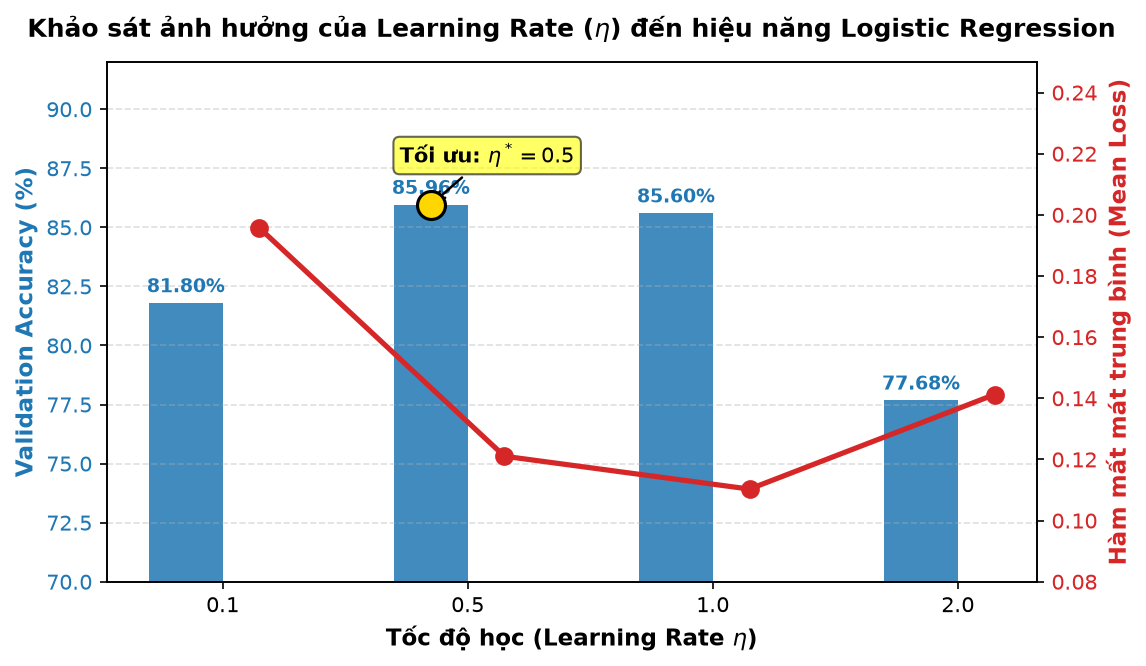
\includegraphics[width=\textwidth]{2_01_logistic_tuning.png}
        \caption{Khảo sát tốc độ học $\eta$ trên tập Validation.}
        \label{fig:lr_tuning}
    \end{subfigure}
    \hfill
    \begin{subfigure}[b]{0.44\textwidth}
        \centering
        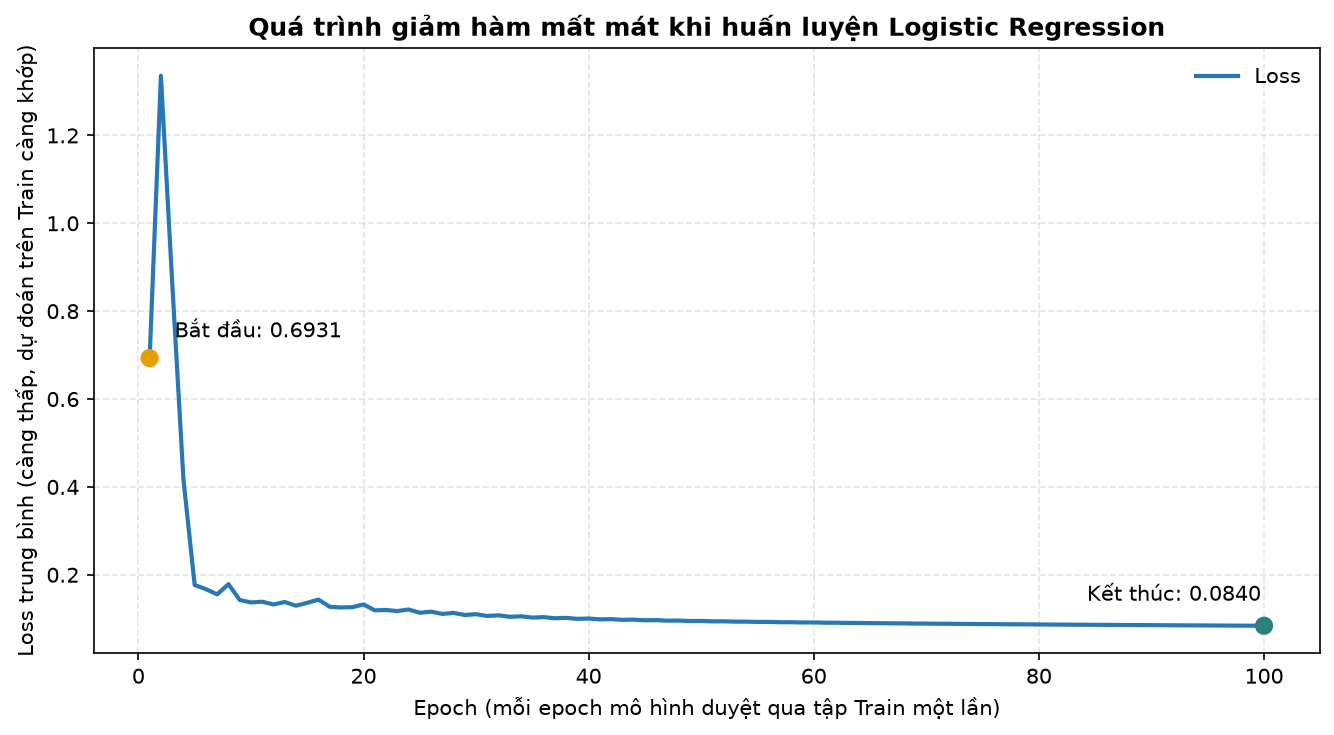
\includegraphics[width=\textwidth]{2_02_logistic_loss_curve.png}
        \caption{Đường cong suy giảm hàm mất mát.}
        \label{fig:lr_loss}
    \end{subfigure}
    \caption{Thực nghiệm tinh chỉnh siêu tham số và động học hội tụ của Logistic Regression.}
    \label{fig:lr_tuning_loss}
\end{figure}

\begin{figure}[H]
    \centering
    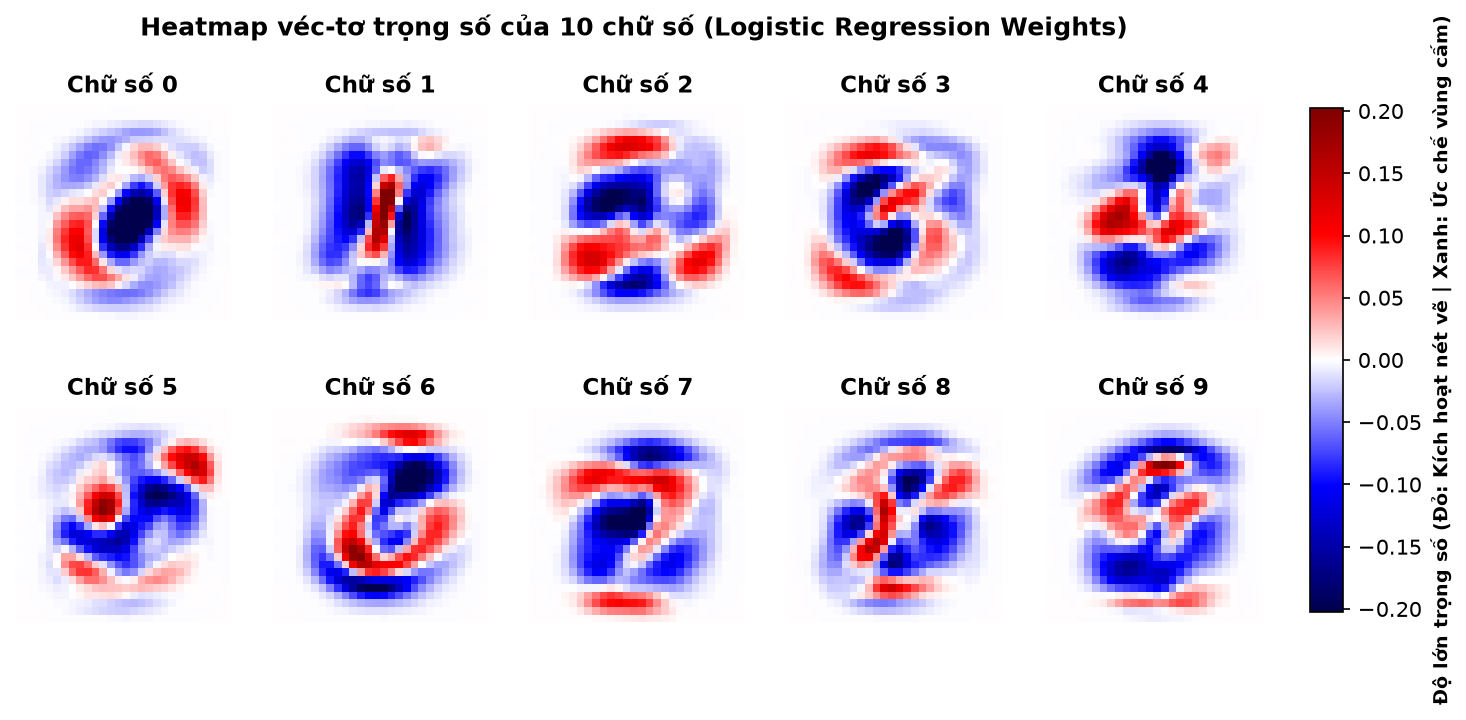
\includegraphics[width=0.70\textwidth]{2_03_logistic_weights.png}
    \caption{Bản đồ nhiệt ma trận trọng số $\mathbf{W}$ ($28 \times 28$) của 10 chữ số.}
    \label{fig:lr_weights}
\end{figure}
\noindent
\textbf{Phân tích bản đồ nhiệt trọng số (Hình~\ref{fig:lr_weights}):}
Mỗi lớp chữ số tương ứng với một ma trận trọng số $28 \times 28$, phản ánh cơ chế ra quyết định của mô hình:
\begin{itemize}[noitemsep]
    \item \textbf{Vùng trọng số dương ($w_j > 0$):} Đóng vai trò kích hoạt. Điểm ảnh có nét mực rơi vào vùng này sẽ làm tăng xác suất dự đoán (ví dụ: viền ngoài của số 0, nét thẳng của số 1).
    \item \textbf{Vùng trọng số âm ($w_j < 0$):} Đóng vai trò ức chế. Nét mực xuất hiện tại đây sẽ làm giảm mạnh điểm số của lớp (ví dụ: phần tâm rỗng của số 0 mang trọng số âm lớn, giúp phân biệt rõ với các số có nét cắt qua tâm như 1, 4, 8).
\end{itemize}
Ngoài ra, điều chuẩn $L_2$ ($\lambda = 10^{-4}$) giúp trường trọng số phân bổ liền mạch, hạn chế hiện tượng nhiễu cục bộ giữa các pixel lân cận.


\textbf{Đối chiếu Scikit-Learn:} Kiểm chứng với \texttt{OneVsRestClassifier} từ thư viện Scikit-Learn cho kết quả tương đương với Test Accuracy đạt $90.59\%$ (so với $86.84\%$ của mô hình tự cài đặt) và tỷ lệ đồng thuận dự đoán đạt \textbf{89.62\%}, khẳng định tính tin cậy của thuật toán cài đặt.

\begin{table}[H]
\centering
\small
\caption{Kết quả thực nghiệm của One-vs-Rest Logistic Regression ($\eta^* = 0.5$, 30 epochs).}
\label{tab:logistic_results}
\resizebox{0.92\textwidth}{!}{%
\begin{tabular}{lrrrrrr}
\toprule
\textbf{Tập dữ liệu} & \textbf{Số mẫu} & \textbf{Accuracy (\%)} & \textbf{Precision (\%)} & \textbf{Recall (\%)} & \textbf{Macro F1 (\%)} & \textbf{Thời gian (s)} \\
\midrule
Train & 50.000 & 86.00 & 86.04 & 85.72 & 85.71 & 10.70 \\
Validation & 10.000 & 85.96 & 85.96 & 85.64 & 85.69 & \textbf{0.03} \\
Test & 10.000 & \textbf{86.84} & 86.87 & 86.58 & 86.55 & \textbf{0.03} \\
\bottomrule
\end{tabular}%
}
\end{table}

\begin{figure}[H]
    \centering
    \begin{subfigure}[b]{0.48\textwidth}
        \centering
        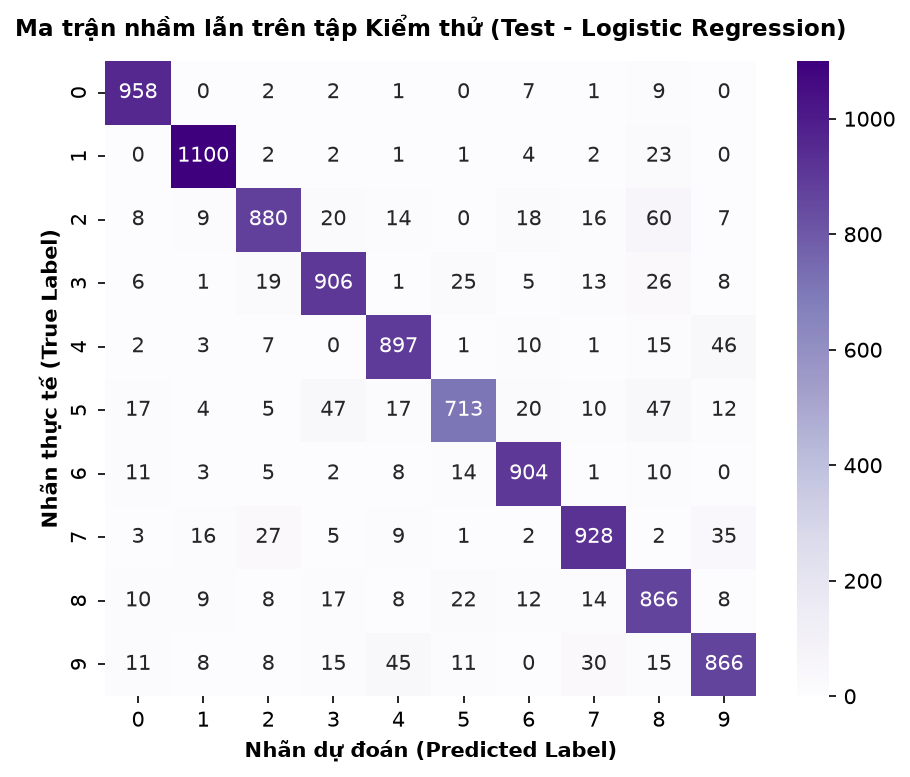
\includegraphics[width=\textwidth]{2_06_logistic_confusion_test.png}
        \caption{LR (OvR) Confushion Test (Acc = 86.84\%).}
        \label{fig:lr_cm}
    \end{subfigure}
    \hfill
    \begin{subfigure}[b]{0.48\textwidth}
        \centering
        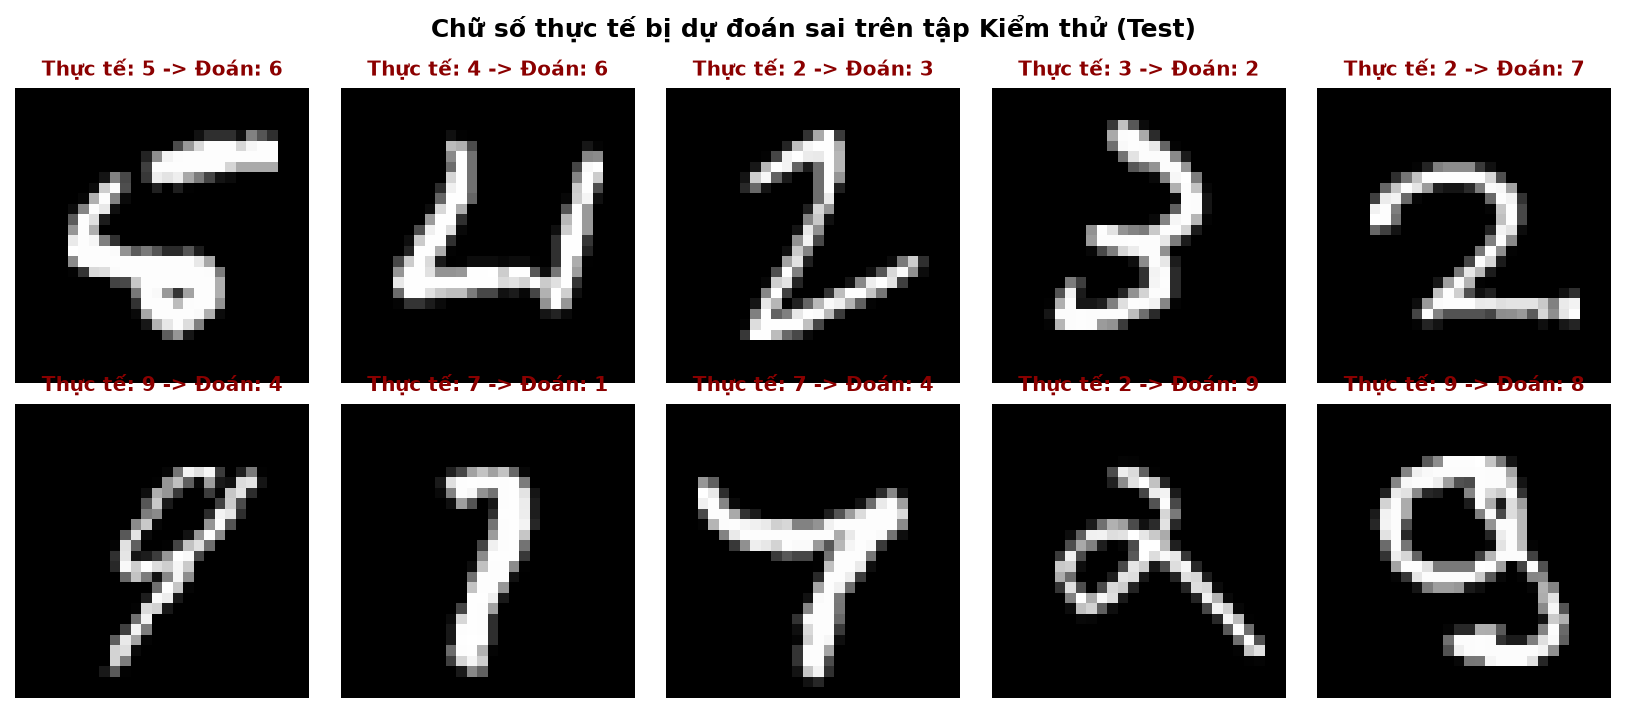
\includegraphics[width=\textwidth]{2_07_logistic_misclassified_samples.png}
        \caption{Các mẫu ảnh bị nhận diện sai điển hình.}
        \label{fig:lr_errors}
    \end{subfigure}
    \caption{Ma trận nhầm lẫn và các trường hợp lỗi phân loại của Logistic Regression.}
    \label{fig:lr_cm_errors}
\end{figure}

\noindent
\textbf{Nhận xét kết quả thực nghiệm:}
\begin{itemize}[noitemsep]
    \item \textbf{Hiệu năng tổng thể:} Độ chính xác trên tập kiểm thử đạt \textbf{86.84\%} (tăng $3.28\%$ so với Naïve Bayes) nhờ cơ chế tối ưu phân biệt và khả năng ức chế bằng trọng số âm. Thời gian huấn luyện là $10.70$s và độ trễ suy luận đạt $0.003$ ms/mẫu.
    \item \textbf{Kết quả theo từng lớp:} Mô hình phân loại tốt nhất ở số 0 ($F_1 = 93.66\%$) và số 1 ($F_1 = 93.43\%$). Khó phân biệt nhất là số 5 do Recall thấp ($68.83\%$, bỏ sót 278 mẫu) và số 8 do Precision thấp ($78.18\%$).
    \item \textbf{Phân tích lỗi và hạn chế:} Các nhầm lẫn phổ biến nhất gồm $(5 \to 3)$ với 92 mẫu, $(4 \leftrightarrow 9)$ với 121 mẫu, cùng các cặp $(5 \to 8)$ và $(2 \to 8)$. Hạn chế cốt lõi nằm ở ranh giới quyết định tuyến tính, không thể nắm bắt được độ nghiêng và cấu trúc phi tuyến phức tạp (Hình~\ref{fig:lr_errors}), dẫn đến nhu cầu áp dụng các mô hình phi tuyến như \textbf{MLP} và \textbf{CNN}.
\end{itemize}

\section{Mô hình 3: Multi-Layer Perceptron (MLP) và Convolutional Neural Network (CNN)}

\subsection{Mạng nơ-ron truyền thẳng nhiều tầng (MLP)}

Mô hình Multi-Layer Perceptron (MLP) giải quyết bài toán phân loại chữ số bằng cách kết hợp các phép biến đổi tuyến tính với hàm kích hoạt phi tuyến ReLU. Nhóm sử dụng kiến trúc baseline $784 \to 256 \to 128 \to 10$, trong đó ma trận trọng số được khởi tạo theo phân phối He.

Ở chiều lan truyền thuận, dữ liệu đi qua các tầng ẩn kết hợp kỹ thuật Inverted Dropout để chống quá khớp. Tại tầng ra, các điểm số logits được chuẩn hóa thành xác suất dự đoán $\hat{\mathbf{Y}}$ qua hàm Softmax.

Quá trình lan truyền ngược tối ưu hàm mất mát Cross-Entropy bắt đầu từ sai số tầng ra:
\begin{equation}
    \boldsymbol{\Delta}^{(L)} = \frac{\hat{\mathbf{Y}} - \mathbf{Y}}{N}
\end{equation}
Tín hiệu sai số được truyền ngược lần lượt qua các tầng ẩn theo đạo hàm ReLU. Nhờ kỹ thuật vector hóa ma trận, gradient của trọng số và bias tại mỗi tầng được tính toán song song kết hợp điều chuẩn $L_2$ ($\lambda = 10^{-4}$):
\begin{equation}
    \frac{\partial J_{\text{reg}}}{\partial \mathbf{W}^{(l)}} = (\boldsymbol{\Delta}^{(l)})^T \mathbf{A}^{(l-1)} + \lambda \mathbf{W}^{(l)}, \quad \frac{\partial J}{\partial \mathbf{b}^{(l)}} = \sum_{i=1}^N \boldsymbol{\Delta}_i^{(l)}
\end{equation}

Mạng được huấn luyện theo từng mini-batch bằng giải thuật SGD có động lượng (Momentum). Đồng thời, cơ chế Early Stopping được áp dụng để theo dõi \texttt{val\_loss}: nếu sau 4 epoch liên tiếp mất mát kiểm định không cải thiện, quá trình huấn luyện sẽ dừng sớm và khôi phục trạng thái trọng số tối ưu nhất.

\textbf{Quy trình xử lý (Pipeline):}
\begin{center}
\resizebox{1\textwidth}{!}{%
\begin{tikzpicture}[
    box/.style={
        draw=blue!70!black,
        fill=blue!4,
        rounded corners=6pt,
        line width=1.1pt,
        text width=4.6cm,
        minimum height=3.8cm,
        align=center,
        inner sep=6pt,
        font=\small
    },
    flow/.style={
        -{Stealth[length=3mm]},
        line width=1.3pt,
        draw=blue!80!black
    },
    backflow/.style={
        -{Stealth[length=3mm]},
        line width=1.3pt,
        draw=red!75!black
    },
    labeltext/.style={
        font=\footnotesize\bfseries
    },
    node distance=0.8cm
]

% 1. Khối Dữ liệu đầu vào
\node[box] (input) {
    \textbf{\textcolor{blue!80!black}{\large 1. Biểu diễn đầu vào}}\\[5pt]
    $\mathbf{x} \in \mathbb{R}^{784}$ (từ ảnh $28 \times 28$)\\[4pt]
    \textbf{Chuẩn hóa Z-score:}\\
    $\mathbf{a}^{(0)} = \frac{\mathbf{x} - \mu}{\sigma + \epsilon}$\\[5pt]
    \textbf{Mini-batch:} $\mathbf{X}_B \in \mathbb{R}^{B \times 784}$
};

% 2. Khối Lan truyền xuôi (MLP Architecture)
\node[box, right=of input] (forward) {
    \textbf{\textcolor{blue!80!black}{\large 2. Lan truyền xuôi}}\\[5pt]
    Khởi tạo He: $\mathbf{W}^{(l)} \sim \mathcal{N}\left(0, \sqrt{\frac{2}{n_{l-1}}}\right)$\\[4pt]
    $\mathbf{Z}^{(l)} = \mathbf{A}^{(l-1)}(\mathbf{W}^{(l)})^T + \mathbf{b}^{(l)}$\\[3pt]
    $\mathbf{A}^{(l)} = \max\left(0, \mathbf{Z}^{(l)}\right) \odot \frac{\mathbf{M}}{1 - p}$\\[4pt]
    $\hat{\mathbf{Y}} = \text{softmax}\left(\mathbf{Z}^{(L)}\right) \in [0, 1]^{B \times 10}$
};

% 3. Khối Hàm mất mát & Gradient tầng ra
\node[box, right=of forward] (loss) {
    \textbf{\textcolor{blue!80!black}{\large 3. Mất mát \& Gradient ra}}\\[5pt]
    \textbf{Cross-Entropy + $L_2$:}\\
    $J = -\frac{1}{B}\sum \ln \hat{y}_{i, c} + \frac{\lambda}{2}\sum \|\mathbf{W}^{(l)}\|_F^2$\\[6pt]
    \textbf{Gradient sai số tầng ra (BP1):}\\
    $\boldsymbol{\Delta}^{(L)} = \frac{\hat{\mathbf{Y}} - \mathbf{Y}}{B}$
};

% 4. Khối Lan truyền ngược & Cập nhật tham số
\node[box, right=of loss] (backward) {
    \textbf{\textcolor{blue!80!black}{\large 4. Lan truyền ngược \& Tối ưu}}\\[5pt]
    \textbf{Đạo hàm ẩn (BP2):}\\
    $\boldsymbol{\Delta}^{(l)} = \mathbf{G}^{(l)} \odot (\mathbf{Z}^{(l)} > 0)$\\[4pt]
    $\nabla_{\mathbf{W}^{(l)}} J = (\boldsymbol{\Delta}^{(l)})^T \mathbf{A}^{(l-1)} + \lambda \mathbf{W}^{(l)}$\\[4pt]
    \textbf{SGD Momentum:}\\
    $\mathbf{v} \leftarrow \beta \mathbf{v} - \eta \nabla_{\mathbf{W}} J, \quad \mathbf{W} \leftarrow \mathbf{W} + \mathbf{v}$
};

% Mũi tên lan truyền thuận (Forward Pass)
\draw[flow] (input.east) -- (forward.west);
\draw[flow] (forward.east) -- (loss.west);
\draw[flow] (loss.east) -- (backward.west);

% Nhãn Forward Pass ở phía trên
\path (input.north west) -- (backward.north east) 
    node[midway, above=6pt, labeltext, text=green!55!black] 
    {Lan truyền thuận (Forward Pass: $784 \to 256 \to 128 \to 10$) $\xrightarrow{\hspace*{3cm}}$};

% Đường lặp ngược tối ưu tham số (Backward Pass loop)
\draw[backflow] (backward.south) -- ++(0,-0.6) -| (forward.south)
    node[pos=0.25, below=2pt, labeltext, text=red!75!black] 
    {$\xleftarrow{\hspace*{2.5cm}}$ Lan truyền ngược (Backward Pass) \& Cập nhật trọng số};

\end{tikzpicture}%
}
\end{center}

Thuật toán MLP được mô tả chi tiết trong Thuật toán 3.

\begin{algorithm}[H]
\caption{Huấn luyện Mạng nơ-ron nhiều tầng (MLP Backpropagation with Momentum)}
\label{alg:mlp_backprop}
\begin{algorithmic}[1]
\Require Dữ liệu $\mathbf{X}$, nhãn $\mathbf{y}$, số tầng $L$, tốc độ học $\eta$, hệ số quán tính $\beta$, batch size $B$.
\Ensure Tập trọng số và độ lệch tối ưu $\{\mathbf{W}^{(l)}, \mathbf{b}^{(l)}\}_{l=1}^L$.
\State Khởi tạo trọng số He $\mathbf{W}^{(l)} \sim \mathcal{N}(0, \sqrt{2/n_{l-1}})$, bias $\mathbf{b}^{(l)} \leftarrow \mathbf{0}$, vận tốc $\mathbf{v}^{(l)} \leftarrow \mathbf{0}$.
\For{mỗi mini-batch $(\mathbf{X}_B, \mathbf{Y}_B)$}
    \State \textbf{Forward:} $\mathbf{z}^{(l)} = \mathbf{W}^{(l)}\mathbf{a}^{(l-1)} + \mathbf{b}^{(l)}$, $\mathbf{a}^{(l)} = \text{ReLU}(\mathbf{z}^{(l)})$; tầng cuối Softmax $\mathbf{P} = \text{softmax}(\mathbf{z}^{(L)})$.
    \State \textbf{Backward:} Lỗi tầng ra $\boldsymbol{\delta}^{(L)} = \mathbf{P} - \mathbf{T}$; lỗi tầng ẩn $\boldsymbol{\delta}^{(l)} = [(\mathbf{W}^{(l+1)})^T \boldsymbol{\delta}^{(l+1)}] \odot \mathbf{1}(\mathbf{z}^{(l)} > 0)$.
    \State \textbf{Update:} $\mathbf{v}^{(l)} \leftarrow \beta \mathbf{v}^{(l)} + \eta \left( \frac{1}{B}\boldsymbol{\delta}^{(l)}(\mathbf{a}^{(l-1)})^T + \lambda\mathbf{W}^{(l)} \right)$, $\mathbf{W}^{(l)} \leftarrow \mathbf{W}^{(l)} - \mathbf{v}^{(l)}$.
\EndFor
\State \Return $\{\mathbf{W}^{(l)}, \mathbf{b}^{(l)}\}_{l=1}^L$
\end{algorithmic}
\end{algorithm}

\subsection{Thí nghiệm với các tham số MLP}

Từ mô hình baseline ban đầu ($784 \to 256 \to 128 \to 10$, ReLU, khởi tạo He, $\gamma = 0.05$, $\alpha = 0.9$, batch size $128$, đạt Val Accuracy $97.77\%$), nhóm tiến hành thực nghiệm đơn biến trên tập Validation (10 epoch/cấu hình) để xác định bộ siêu tham số tối ưu.

\textbf{a. Tốc độ học ($\gamma$) và Quán tính ($\alpha$):} Khảo sát lưới $\gamma \in \{0.005, 0.01, 0.05, 0.1, 0.5\}$ và $\alpha \in \{0.0, 0.5, 0.9\}$ với tốc độ học hiệu dụng $\gamma_{\text{eff}} = \frac{\gamma}{1 - \alpha}$.

\begin{figure}[H]
    \centering
    \begin{minipage}{0.6\linewidth}
        \centering
        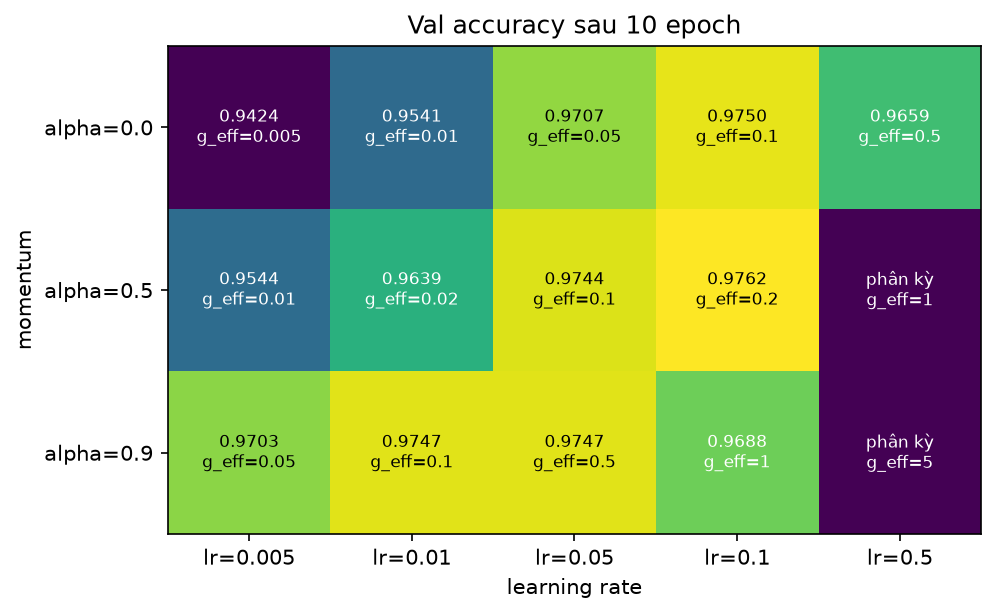
\includegraphics[width=\linewidth]{3_02_hyperparameter_lr_momentum.png}
        \caption{Khảo sát Learning rate và Momentum}
        \label{fig:mlp_lr_mom}
    \end{minipage}
\end{figure}

\textbf{b. Kích thước Mini-batch và Kiến trúc mạng:} Cố định cặp tham số tốt nhất từ bước 1 ($\gamma = 0.1, \alpha = 0.5$), nhóm lần lượt khảo sát kích thước batch và 5 cấu hình độ rộng/sâu của mạng:

\begin{table}[H]
    \centering
    \footnotesize
    \begin{tabular}{|c|c|c|c|}
        \hline
        \textbf{Batch} & \textbf{Cập nhật} & \textbf{Giây/ep} & \textbf{Val Acc} \\
        \hline
        16 & 15.625 & 3.97s & 96.11\% \\
        \textbf{64} & \textbf{3.910} & \textbf{1.57s} & \textbf{97.94\%} \\
        256 & 980 & 0.72s & 97.37\% \\
        1024 & 245 & 0.49s & 96.60\% \\
        \hline
    \end{tabular}
    \quad
    \begin{tabular}{|l|c|c|c|}
        \hline
        \textbf{Kiến trúc mạng} & \textbf{Tham số} & \textbf{Train} & \textbf{Val Acc} \\
        \hline
        $784 \to 64 \to 10$ & 50.890 & 99.37\% & 97.12\% \\
        $784 \to 256 \to 10$ & 203.530 & 100\% & 97.63\% \\
        $784 \to 1024 \to 10$ & 814.090 & 100\% & 97.90\% \\
        $\mathbf{784 \to 256 \to 128 \to 10}$ & \textbf{235.146} & \textbf{100\%} & \textbf{97.94\%} \\
        $784 \to 256^4 \to 10$ & 400.906 & 99.38\% & 97.30\% \\
        \hline
    \end{tabular}
\end{table}

\textbf{c. Hàm kích hoạt và Khởi tạo trọng số:} Đo chuẩn Frobenius $\|\partial J / \partial \mathbf{W}^{(l)}\|_F$ qua 6 lớp ẩn ($784 \to 128^6 \to 10$) và độ lệch chuẩn tín hiệu ($\text{std}$) qua 10 lớp ReLU ($784 \to 256^{10} \to 10$):

\begin{figure}[H]
    \centering
    \begin{minipage}{0.48\linewidth}
        \centering
        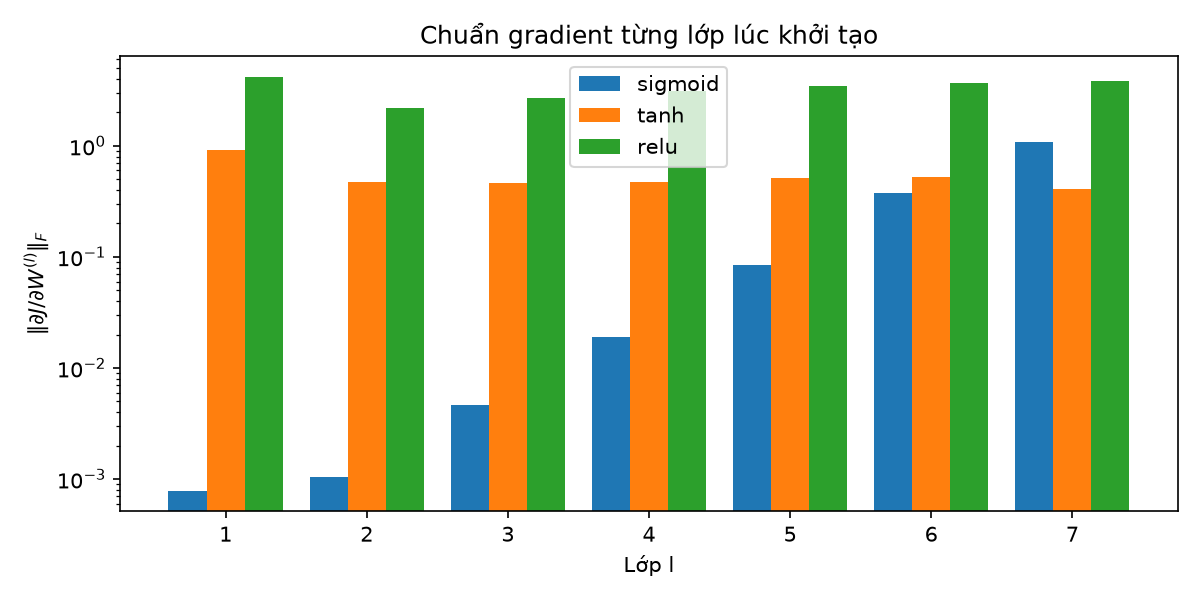
\includegraphics[width=\linewidth]{3_03_vanishing_gradient.png}
        \caption{Chuẩn gradient theo hàm kích hoạt}
        \label{fig:mlp_grad}
    \end{minipage}\hfill
    \begin{minipage}{0.48\linewidth}
        \centering
        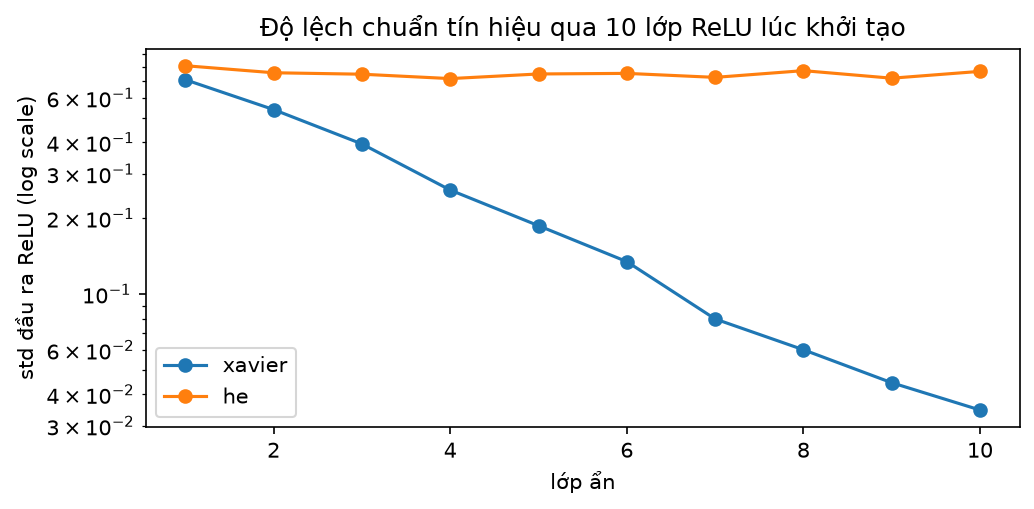
\includegraphics[width=\linewidth]{3_04_variance_preservation.png}
        \caption{Độ lệch chuẩn tín hiệu qua 10 lớp ReLU}
        \label{fig:mlp_std}
    \end{minipage}
\end{figure}

\noindent
\textbf{Nhận xét và Lựa chọn cấu hình tối ưu:}
\begin{itemize}[noitemsep]
    \item \textbf{Siêu tham số huấn luyện:} Cặp $(\gamma = 0.1, \alpha = 0.5)$ giúp hội tụ ổn định, tránh hiện tượng phân kỳ (\texttt{NaN}) khi $\gamma = 0.5, \alpha \ge 0.5$. Kết hợp cùng \textbf{batch size 64}, mô hình đạt độ chính xác kiểm định cao nhất (\textbf{97.94\%}) với tốc độ hợp lý (1.57s/epoch).
    \item \textbf{Kiến trúc và Khởi tạo:} Cấu trúc $\mathbf{784 \to 256 \to 128 \to 10}$ (235.146 tham số) cho hiệu năng tốt hơn mạng rộng 1024 nút và mạng sâu 4 lớp ẩn. Việc kết hợp \textbf{ReLU và khởi tạo He} giúp khắc phục triệt để hiện tượng tiêu biến gradient của Sigmoid (suy giảm 1.400 lần) và suy giảm phương sai của Xavier.
\end{itemize}
\subsection{Mạng nơ-ron tích chập (CNN) và So sánh đánh giá}

Khác với MLP làm phẳng ảnh khiến cấu trúc lân cận bị phá vỡ, mạng tích chập (CNN) giữ nguyên đầu vào dạng tensor 2D $\mathbf{X} \in [0, 1]^{1 \times 28 \times 28}$ để khai thác trực tiếp tương quan không gian cục bộ (nét bút, góc cạnh).

Tại tầng tích chập (Conv2D), $32$ bộ lọc $\mathbf{K}_k$ kích thước $4 \times 4$ ($s = 1, p = 0$) trượt trên ảnh để trích xuất bản đồ đặc trưng và kích hoạt qua hàm ReLU:
\begin{equation}
    z_{k,i,j} = \sum_{c,u,v} K_{k,c,u,v} \, x_{c, i+u, j+v} + b_k, \qquad a_{k,i,j} = \text{ReLU}(z_{k,i,j})
\end{equation}
Tiếp theo, tầng gộp cực đại (Max-Pooling $2 \times 2, s = 2$) giữ lại đặc trưng nổi bật nhất trong từng vùng cục bộ, giúp giảm một nửa kích thước không gian và tăng tính bất biến dịch chuyển:
\begin{equation}
    p_{k,i,j} = \max_{(u,v) \in \{0,1\}^2} a_{k, 2i+u, 2j+v}
\end{equation}
Bản đồ đặc trưng $(12 \times 12 \times 32)$ sau đó được trải phẳng thành vector $4608$ chiều, đi qua tầng kết nối đầy đủ (Dense $128$ + ReLU) và chuẩn hóa bằng hàm Softmax ở tầng ra để dự đoán chữ số $\hat{y} = \arg\max_k P(y = k \mid \mathbf{x})$. Toàn bộ mạng gồm $591.786$ tham số, được huấn luyện bằng bộ tối ưu Adam ($\text{lr} = 10^{-3}$, batch size $128$) kết hợp Early Stopping ($\text{patience} = 2$).

\begin{figure}[H]
\centering
\resizebox{0.82\textwidth}{!}{%
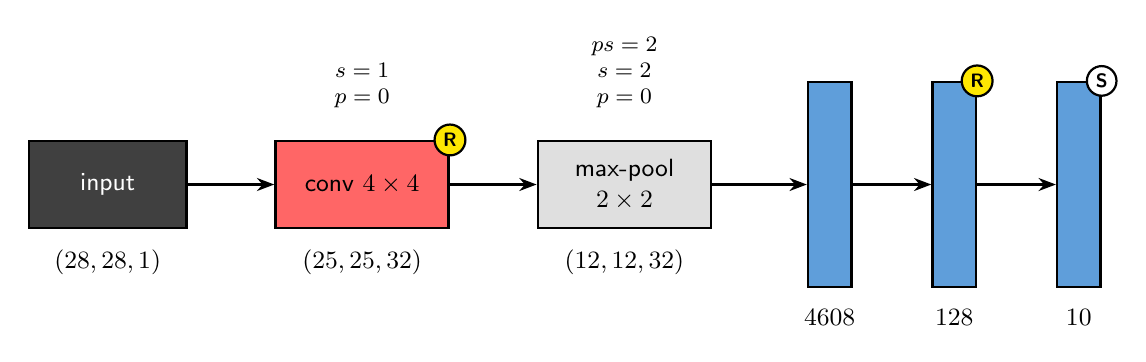
\begin{tikzpicture}[
    font=\sffamily\small,
    arrow/.style={-{Stealth[length=2.2mm]}, line width=0.9pt, draw=black},
    inputbox/.style={draw=black, line width=0.9pt, fill=black!75, text=white, minimum width=2.0cm, minimum height=1.1cm, align=center},
    convbox/.style={draw=black, line width=0.9pt, fill=red!60!white, minimum width=2.2cm, minimum height=1.1cm, align=center},
    poolbox/.style={draw=black, line width=0.9pt, fill=gray!25, minimum width=2.2cm, minimum height=1.1cm, align=center},
    fcbox/.style={draw=black, line width=0.9pt, fill=cyan!60!blue!65, minimum width=0.55cm, minimum height=2.6cm},
    actR/.style={circle, draw=black, line width=0.8pt, fill=yellow!90!orange, inner sep=1.5pt, font=\sffamily\scriptsize\bfseries},
    actS/.style={circle, draw=black, line width=0.8pt, fill=white, inner sep=1.5pt, font=\sffamily\scriptsize\bfseries}
]

% 1. Input
\node[inputbox] (in) {input};
\node[below=4pt of in, font=\small] {$(28, 28, 1)$};

% 2. Conv 4x4
\node[convbox, right=1.1cm of in] (conv) {conv $4\times 4$};
\node[actR] at (conv.north east) {R};
\node[above=8pt of conv, align=center, font=\footnotesize] {$s = 1$\\$p = 0$};
\node[below=4pt of conv, font=\small] {$(25, 25, 32)$};

% 3. Max-Pool 2x2
\node[poolbox, right=1.1cm of conv] (pool) {max-pool\\$2\times 2$};
\node[above=8pt of pool, align=center, font=\footnotesize] {$ps = 2$\\$s = 2$\\$p = 0$};
\node[below=4pt of pool, font=\small] {$(12, 12, 32)$};

% 4. Flatten (4608)
\node[fcbox, right=1.2cm of pool] (flat) {};
\node[below=4pt of flat, font=\small] {$4608$};

% 5. Dense 128 + ReLU
\node[fcbox, right=1.0cm of flat] (fc1) {};
\node[actR] at (fc1.north east) {R};
\node[below=4pt of fc1, font=\small] {$128$};

% 6. Dense 10 + Softmax
\node[fcbox, right=1.0cm of fc1] (fc2) {};
\node[actS] at (fc2.north east) {S};
\node[below=4pt of fc2, font=\small] {$10$};

% Arrows
\draw[arrow] (in) -- (conv);
\draw[arrow] (conv) -- (pool);
\draw[arrow] (pool.east) -- (flat.west);
\draw[arrow] (flat.east) -- (fc1.west);
\draw[arrow] (fc1.east) -- (fc2.west);

\end{tikzpicture}%
}


\caption{Kiến trúc mạng tích chập \texttt{MNISTCNN} (\textbf{R}: kích hoạt ReLU, \textbf{S}: hàm Softmax)}
\label{fig:cnn_pipeline}
\end{figure}


Trong khuôn khổ nghiên cứu này, việc triển khai mạng nơ-ron tích chập (CNN) được xem như một bước tiếp cận mở rộng nhằm làm rõ bản chất hoạt động của mô hình. Nhóm quyết định thiết lập CNN ở cấu hình cơ bản để tạo ra một hệ quy chiếu (baseline) khách quan phục vụ cho công tác đối chứng. Quá trình tinh chỉnh siêu tham số (hyperparameter tuning) chuyên sâu nhằm tối ưu hóa hiệu năng sẽ là định hướng phát triển ở các giai đoạn tiếp theo. 

\begin{table}[H]
    \centering
    % Thu hẹp khoảng cách giữa các cột để chữ bên trong to hơn
    \setlength{\tabcolsep}{3pt} 
    \begin{minipage}{0.49\textwidth}
        \centering
        \caption{Kết quả thực nghiệm của Mạng nơ-ron nhiều tầng (MLP).}
        \label{tab:mlp_results}
        \resizebox{\linewidth}{!}{%
        \begin{tabular}{lrrrrrr}
        \toprule
        \textbf{Tập dữ liệu} & \textbf{Số mẫu} & \textbf{Accuracy (\%)} & \textbf{Precision (\%)} & \textbf{Recall (\%)} & \textbf{Macro F1 (\%)} & \textbf{Thời gian (s)} \\
        \midrule
        Train & 50.000 & 100.00 & 100.00 & 100.00 & 100.00 & 33.57 \\
        Validation & 10.000 & 97.88 & 97.85 & 97.87 & 97.86 & \textbf{0.02} \\
        Test & 10.000 & \textbf{98.26} & 98.25 & 98.24 & 98.25 & \textbf{0.02} \\
        \bottomrule
        \end{tabular}%
        }
    \end{minipage}\hfill
    \begin{minipage}{0.49\textwidth}
        \centering
        \caption{Kết quả thực nghiệm của Mạng nơ-ron tích chập (CNN).}
        \label{tab:cnn_results}
        \resizebox{\linewidth}{!}{%
        \begin{tabular}{lrrrrrr}
        \toprule
        \textbf{Tập dữ liệu} & \textbf{Số mẫu} & \textbf{Accuracy (\%)} & \textbf{Precision (\%)} & \textbf{Recall (\%)} & \textbf{Macro F1 (\%)} & \textbf{Thời gian (s)} \\
        \midrule
        Train & 50.000 & 99.65 & 99.65 & 99.65 & 99.65 & 51.61 \\
        Validation & 10.000 & 98.58 & 98.57 & 98.57 & 98.57 & 0.44 \\
        Test & 10.000 & \textbf{98.76} & 98.77 & 98.75 & 98.76 & \textbf{0.43} \\
        \bottomrule
        \end{tabular}%
        }
    \end{minipage}
\end{table}
\begin{figure}[H]
    \centering
    % Tăng kích thước ảnh lên 48% chiều ngang mỗi hình để to rõ hơn
    \begin{subfigure}[b]{0.48\textwidth}
        \centering
        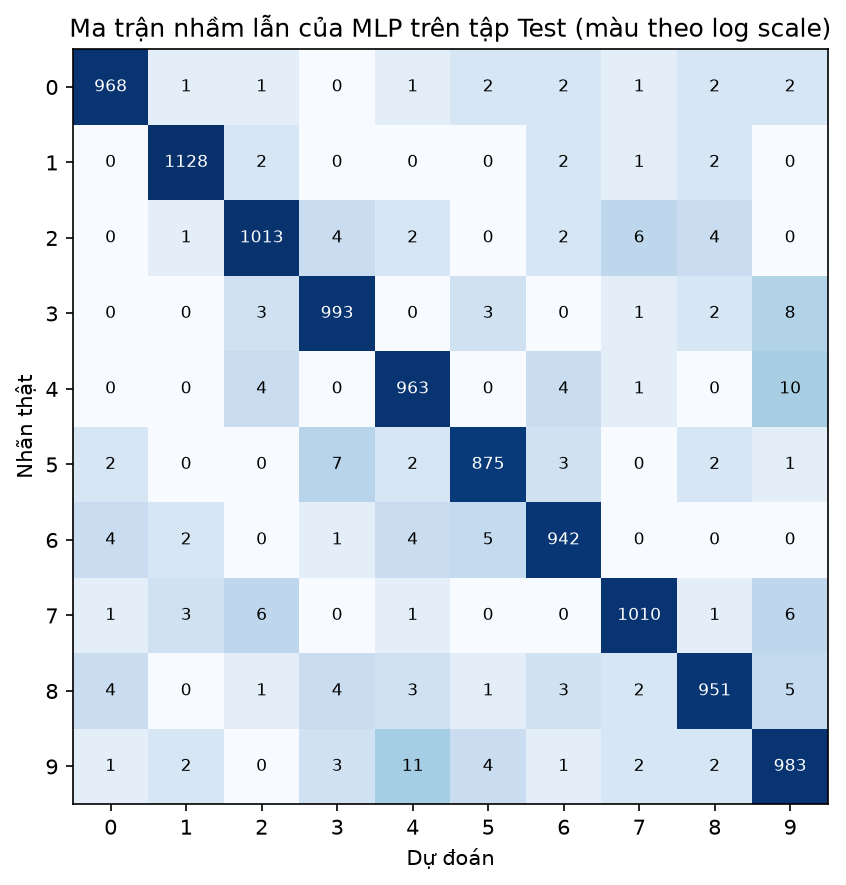
\includegraphics[width=\textwidth]{3_05_mlp_confusion_matrix.png}
        \caption{Ma trận nhầm lẫn MLP (Test Acc = 97.56\%).}
        \label{fig:cm_mlp}
    \end{subfigure}
    \hfill
    \begin{subfigure}[b]{0.48\textwidth}
        \centering
        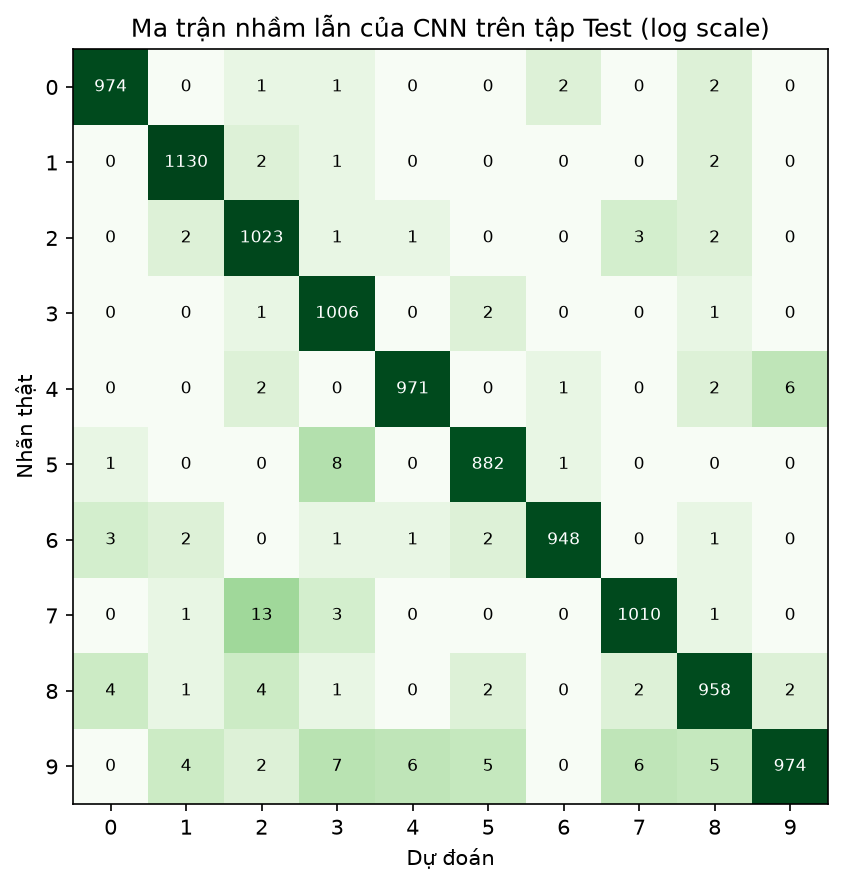
\includegraphics[width=\textwidth]{3_07_cnn_confusion_matrix.png}
        \caption{Ma trận nhầm lẫn CNN (Test Acc = 98.76\%).}
        \label{fig:cm_cnn}
    \end{subfigure}
    \caption{Đối chiếu ma trận nhầm lẫn trên tập Test của MLP và CNN.}
    \label{fig:deep_cm_compare}
\end{figure}

\begin{figure}[H]
    \centering
    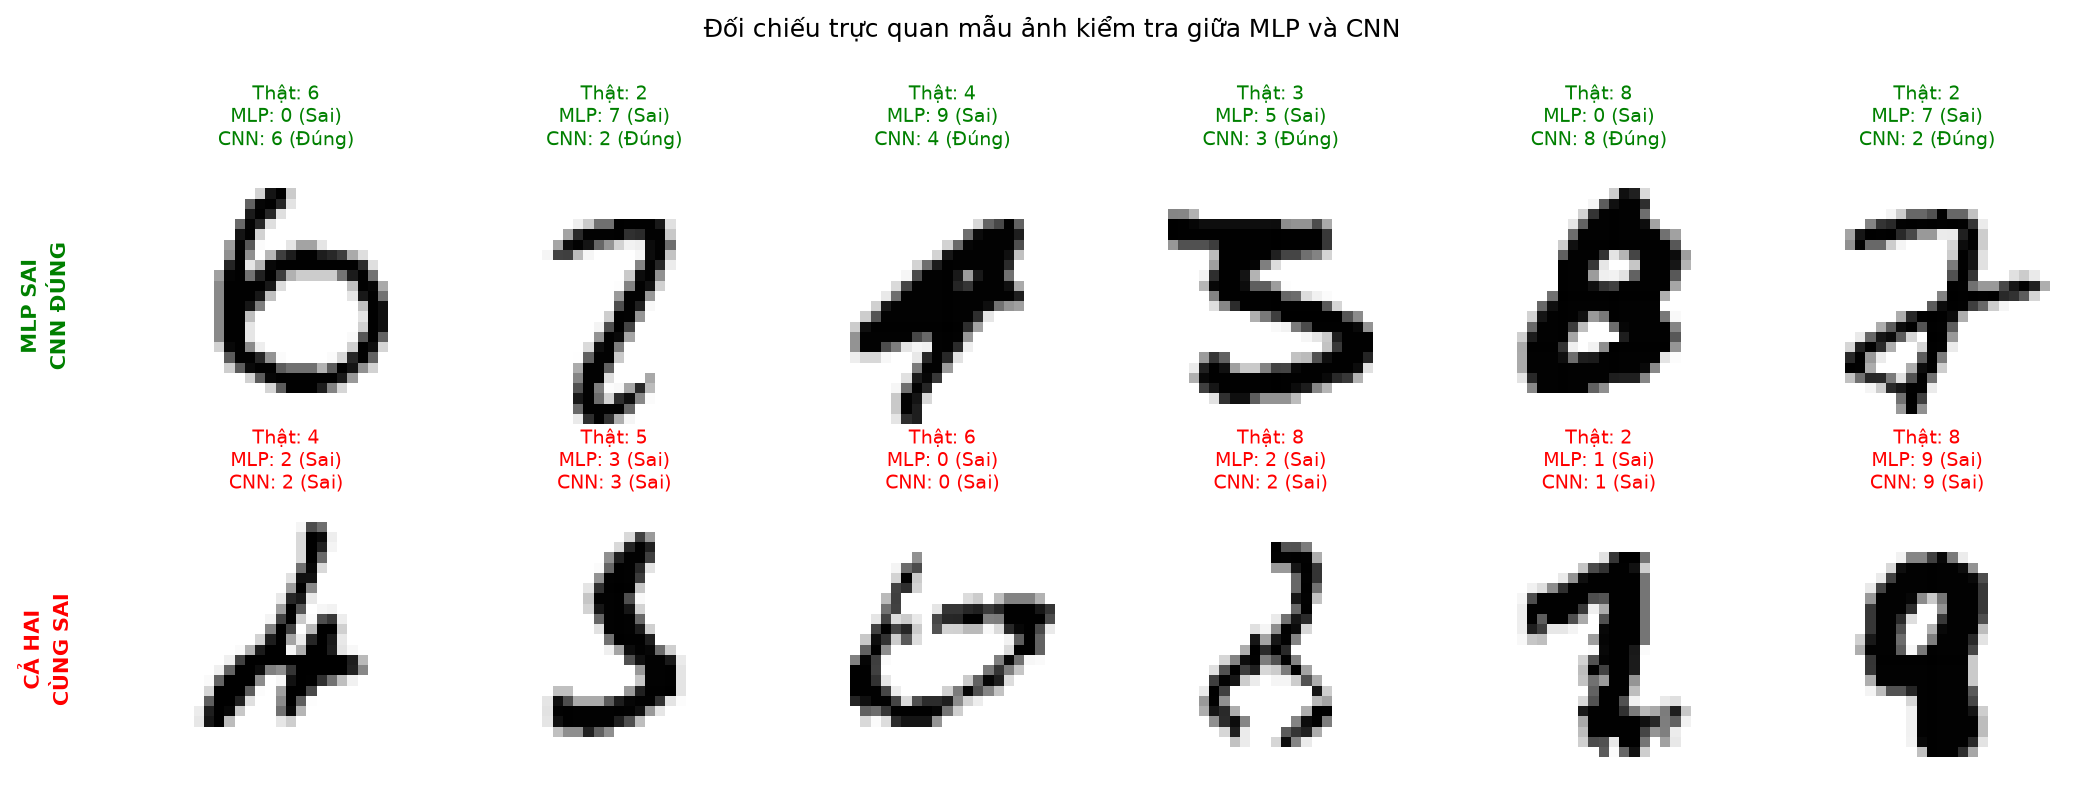
\includegraphics[width=0.7\textwidth]{3_09_mlp_vs_cnn_error_analysis.png}
    \caption{Phân tích các mẫu chữ viết tay mà MLP đoán sai nhưng CNN nhận diện chính xác.}
    \label{fig:cnn_win}
\end{figure}

\noindent
\textbf{So sánh hiệu năng giữa MLP và CNN:}
\begin{itemize}[noitemsep]
    \item \textbf{Độ chính xác:} Trên tập Test (10.000 mẫu), CNN đạt Accuracy \textbf{98.76\%} (124 mẫu sai), vượt trội hơn MLP với \textbf{98.26\%} (174 mẫu sai).
    \item \textbf{Độ phức tạp và Tốc độ:} CNN sở hữu \textbf{591.786 tham số} (gấp 2.5 lần MLP) và thời gian huấn luyện dài hơn ($44$ giây so với $30$ giây của MLP). Đáng chú ý, gần $99.7\%$ tham số của CNN tập trung ở lớp Dense đầu tiên sau Flatten, trong khi lớp tích chập chỉ chiếm $544$ tham số.
\end{itemize}

\textbf{Tóm lại}: Sự chênh lệch này là do cách hai mô hình xử lý dữ liệu. MLP yêu cầu duỗi thẳng ảnh thành một vector 1D, vô tình làm mất đi mối liên hệ không gian giữa các điểm ảnh. Trong khi đó, CNN giữ nguyên cấu trúc lưới 2D của ảnh và dùng các bộ lọc (filter) để trích xuất trực tiếp các đặc trưng cục bộ (đường nét, góc cạnh).


% ==============================================================================
% CHƯƠNG 6: HỌC QUẦN THỂ (ENSEMBLE) VỚI ADABOOST
% ==============================================================================
\newenvironment{algorithmblock}[2]{%
  \par\medskip\noindent\hrule\smallskip
  \textbf{Thuật toán #1} #2\par\smallskip\hrule\smallskip
  \small
}{\par\smallskip\hrule\medskip}

\section{Mô hình 4: Học quần thể (Ensemble) với AdaBoost}

\subsection{Cơ sở lý thuyết thuật toán AdaBoost}
AdaBoost kết hợp tuần tự nhiều bộ phân loại yếu thành mô hình tổng hợp. Sau mỗi vòng, các mẫu bị dự đoán sai được tăng trọng số để những vòng sau tập trung sửa lỗi. Thuật toán 4 trình bày SAMME, biến thể AdaBoost dùng để phân loại trực tiếp 10 lớp MNIST.

\begin{algorithm}[H]
\caption{Huấn luyện Học quần thể AdaBoost đa lớp (SAMME)}
\label{alg:adaboost_samme}
\begin{algorithmic}[1]
\Require Tập dữ liệu $\{(\mathbf{x}_i, y_i)\}_{i=1}^{N}$, số lớp $K$, số vòng $T$, tốc độ học $\eta$.
\Ensure Bộ phân loại tổng hợp $H(\mathbf{x}) = \arg\max_k \sum_{t=1}^{T'} \alpha_t \mathbf{1}[h_t(\mathbf{x}) = k]$.
\State Khởi tạo trọng số mẫu phân bố đều: $w_1(i) = 1/N$, $\forall i \in \{1, \ldots, N\}$.
\For{$t = 1 \to T$}
    \State \textbf{Train:} Huấn luyện $h_t = \arg\min_{h \in \mathcal{H}} \sum_{i=1}^{N} w_t(i) \mathbf{1}[h(\mathbf{x}_i) \neq y_i]$.
    \State \textbf{Evaluate:} Tính sai số có trọng số $\epsilon_t = \sum_{i=1}^{N} w_t(i) \mathbf{1}[h_t(\mathbf{x}_i) \neq y_i]$.
    \If{$\epsilon_t = 0$}
        \State \Return $h_t(\mathbf{x})$ (dừng sớm)
    \EndIf
    \If{$\epsilon_t \geq 1 - 1/K$}
        \State Loại $h_t$ và dừng boosting.
    \EndIf
    \State \textbf{Weight:} Tính trọng số mô hình $\alpha_t = \eta \left[ \ln\left(\frac{1-\epsilon_t}{\epsilon_t}\right) + \ln(K-1) \right]$.
    \State \textbf{Update:} Cập nhật trọng số mẫu $\widetilde{w}_{t+1}(i) = w_t(i) \exp(\alpha_t \mathbf{1}[h_t(\mathbf{x}_i) \neq y_i])$.
    \State Chuẩn hóa: $Z_t = \sum_j \widetilde{w}_{t+1}(j)$, $w_{t+1}(i) = \widetilde{w}_{t+1}(i) / Z_t$.
\EndFor
\State \Return $H(\mathbf{x}) = \arg\max_{k \in \{0, \ldots, K-1\}} \sum_{t=1}^{T'} \alpha_t \mathbf{1}[h_t(\mathbf{x}) = k]$ (với $T' \leq T$ là số vòng thực tế đã huấn luyện).
\end{algorithmic}
\end{algorithm}

\subsection{Khảo sát siêu tham số và đánh giá thực nghiệm AdaBoost}
\subsubsection{Khảo sát Accuracy theo thuật toán phân loại}
Đối chiếu Accuracy của AdaBoost khi sử dụng Decision Tree (depth $=1$), Decision Tree (depth $=3$), Logistic Regression và Gaussian Naive Bayes với \texttt{learning\_rate} $=0{,}5$. Trên Validation, Decision Tree (depth $=3$) đạt cao nhất (91,30\%), tiếp theo là Logistic Regression (84,48\%), Decision Tree (depth $=1$) (77,28\%) và Gaussian Naive Bayes (55,98\%). Kết hợp với khảo sát siêu tham số, chọn depth $=3$, \texttt{n\_estimators} $=200$ và \texttt{learning\_rate} $=0{,}5$ để đánh giá trên tập Test độc lập.

\begin{figure}[H]\centering
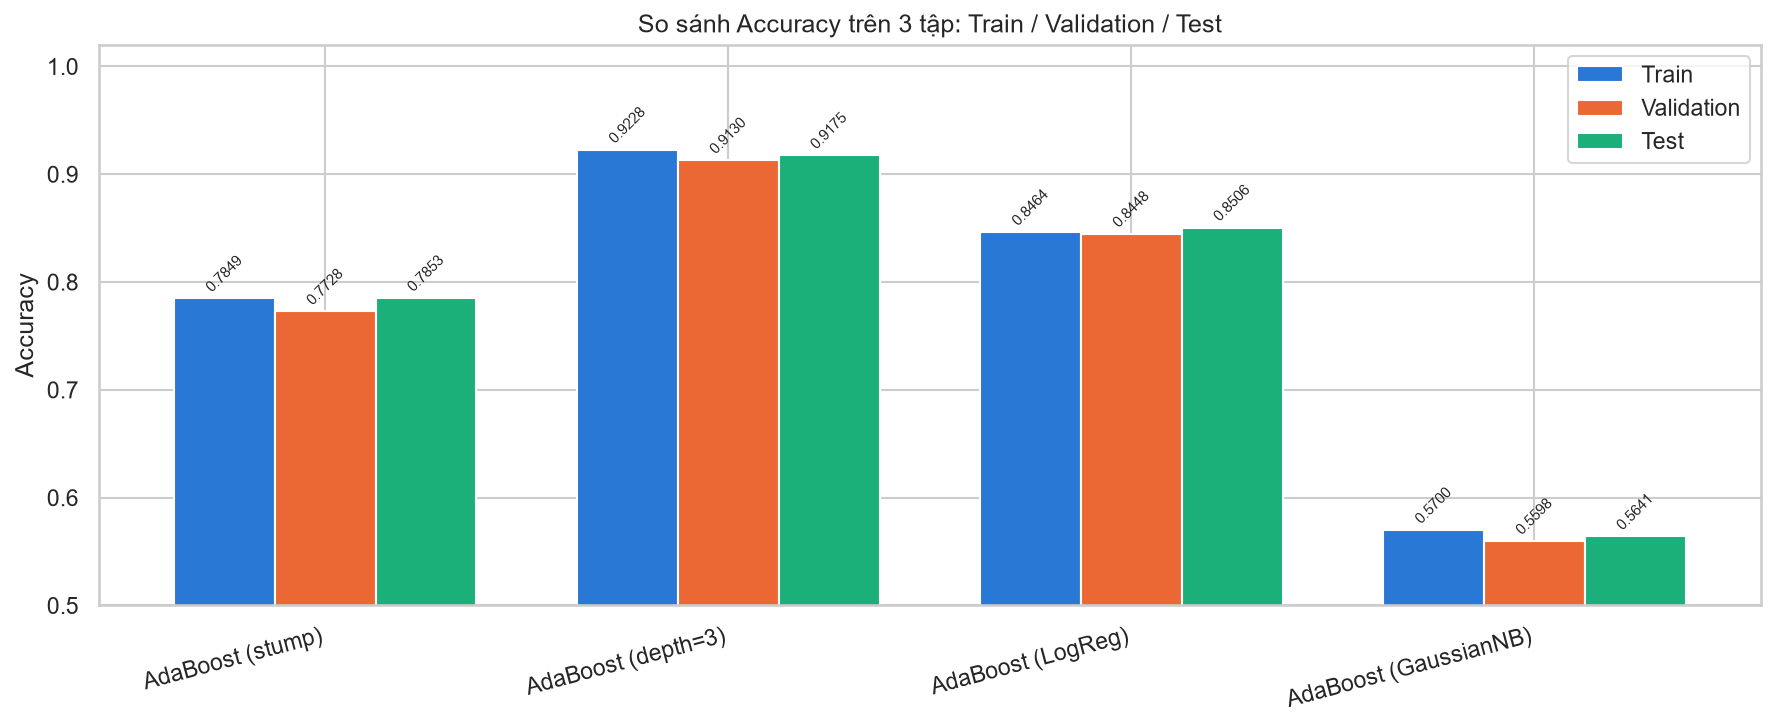
\includegraphics[width=0.9\textwidth]{4_01_accuracy_comparison.png}
\caption{So sánh Accuracy trên Train / Validation / Test.}
\end{figure}

\subsubsection{Khảo sát siêu tham số}
Khảo sát tác động của \texttt{n\_estimators} và \texttt{learning\_rate} đến Accuracy trên 10.000 ảnh Validation sau khi huấn luyện bằng 50.000 ảnh Train. Decision Tree (depth $=3$) dẫn đầu, đạt 91,30\% với 200 vòng boosting; khi cố định 100 vòng, \texttt{learning\_rate} $=0{,}5$ cho kết quả gần 90\%.

\begin{figure}[H]\centering
\begin{subfigure}[b]{0.43\textwidth}\centering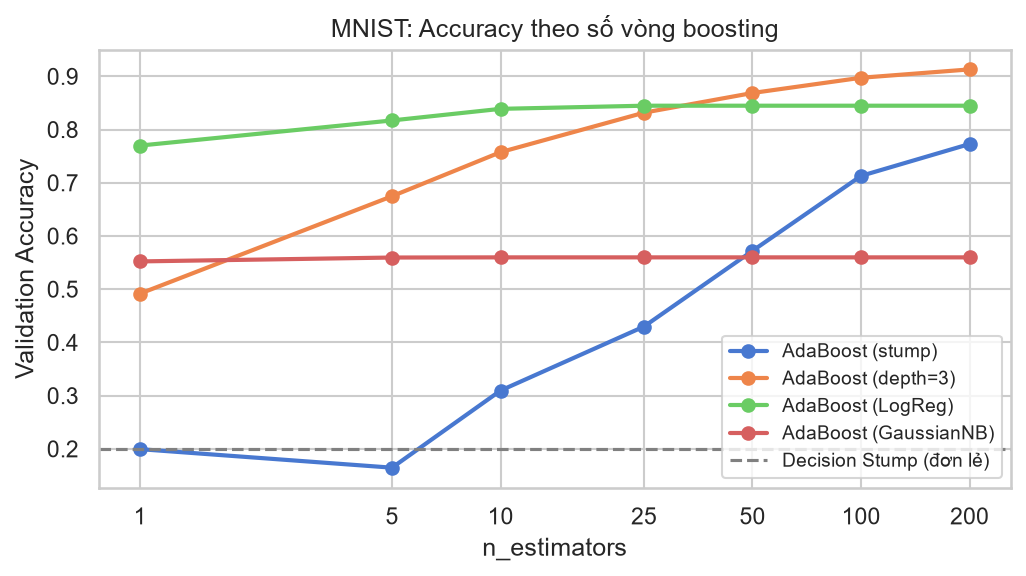
\includegraphics[width=\linewidth]{4_04_n_estimators_analysis.png}\end{subfigure}\hfill
\begin{subfigure}[b]{0.43\textwidth}\centering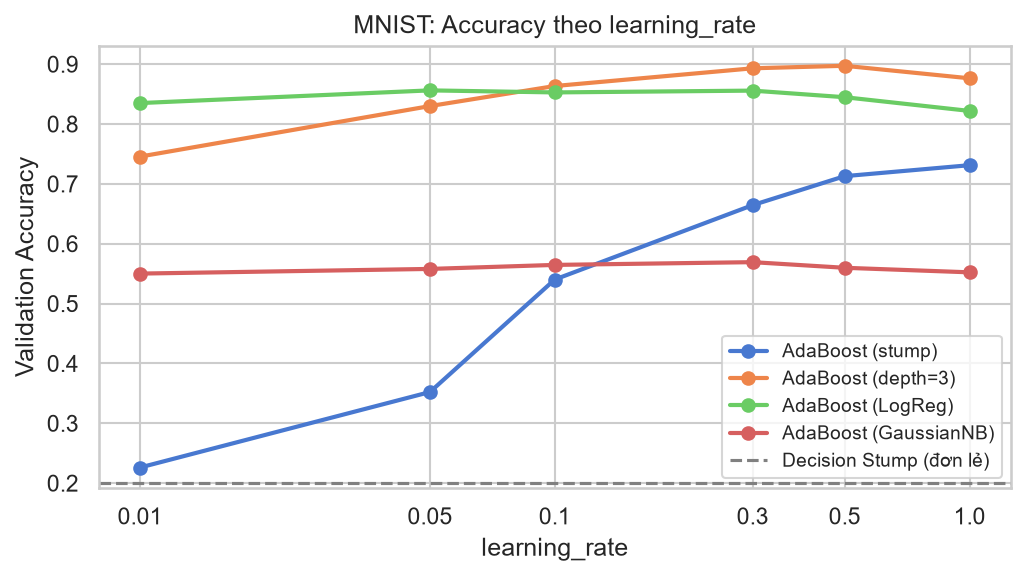
\includegraphics[width=\linewidth]{4_05_learning_rate_analysis.png}\end{subfigure}
\caption{Validation Accuracy theo số vòng boosting (trái) và tốc độ học (phải).}
\end{figure}

\subsubsection{Ma trận nhầm lẫn trên tập kiểm thử}
Ma trận nhầm lẫn đánh giá AdaBoost với Decision Tree (depth $=3$) trên 10.000 ảnh Test độc lập, sau khi chọn tham số bằng Validation. Mô hình đạt Accuracy 91,75\% và Macro-F1 91,70\%; các dự đoán sai tập trung ở những chữ số có nét viết gần nhau, đáng chú ý là cặp 4 và 9.

\begin{figure}[H]\centering
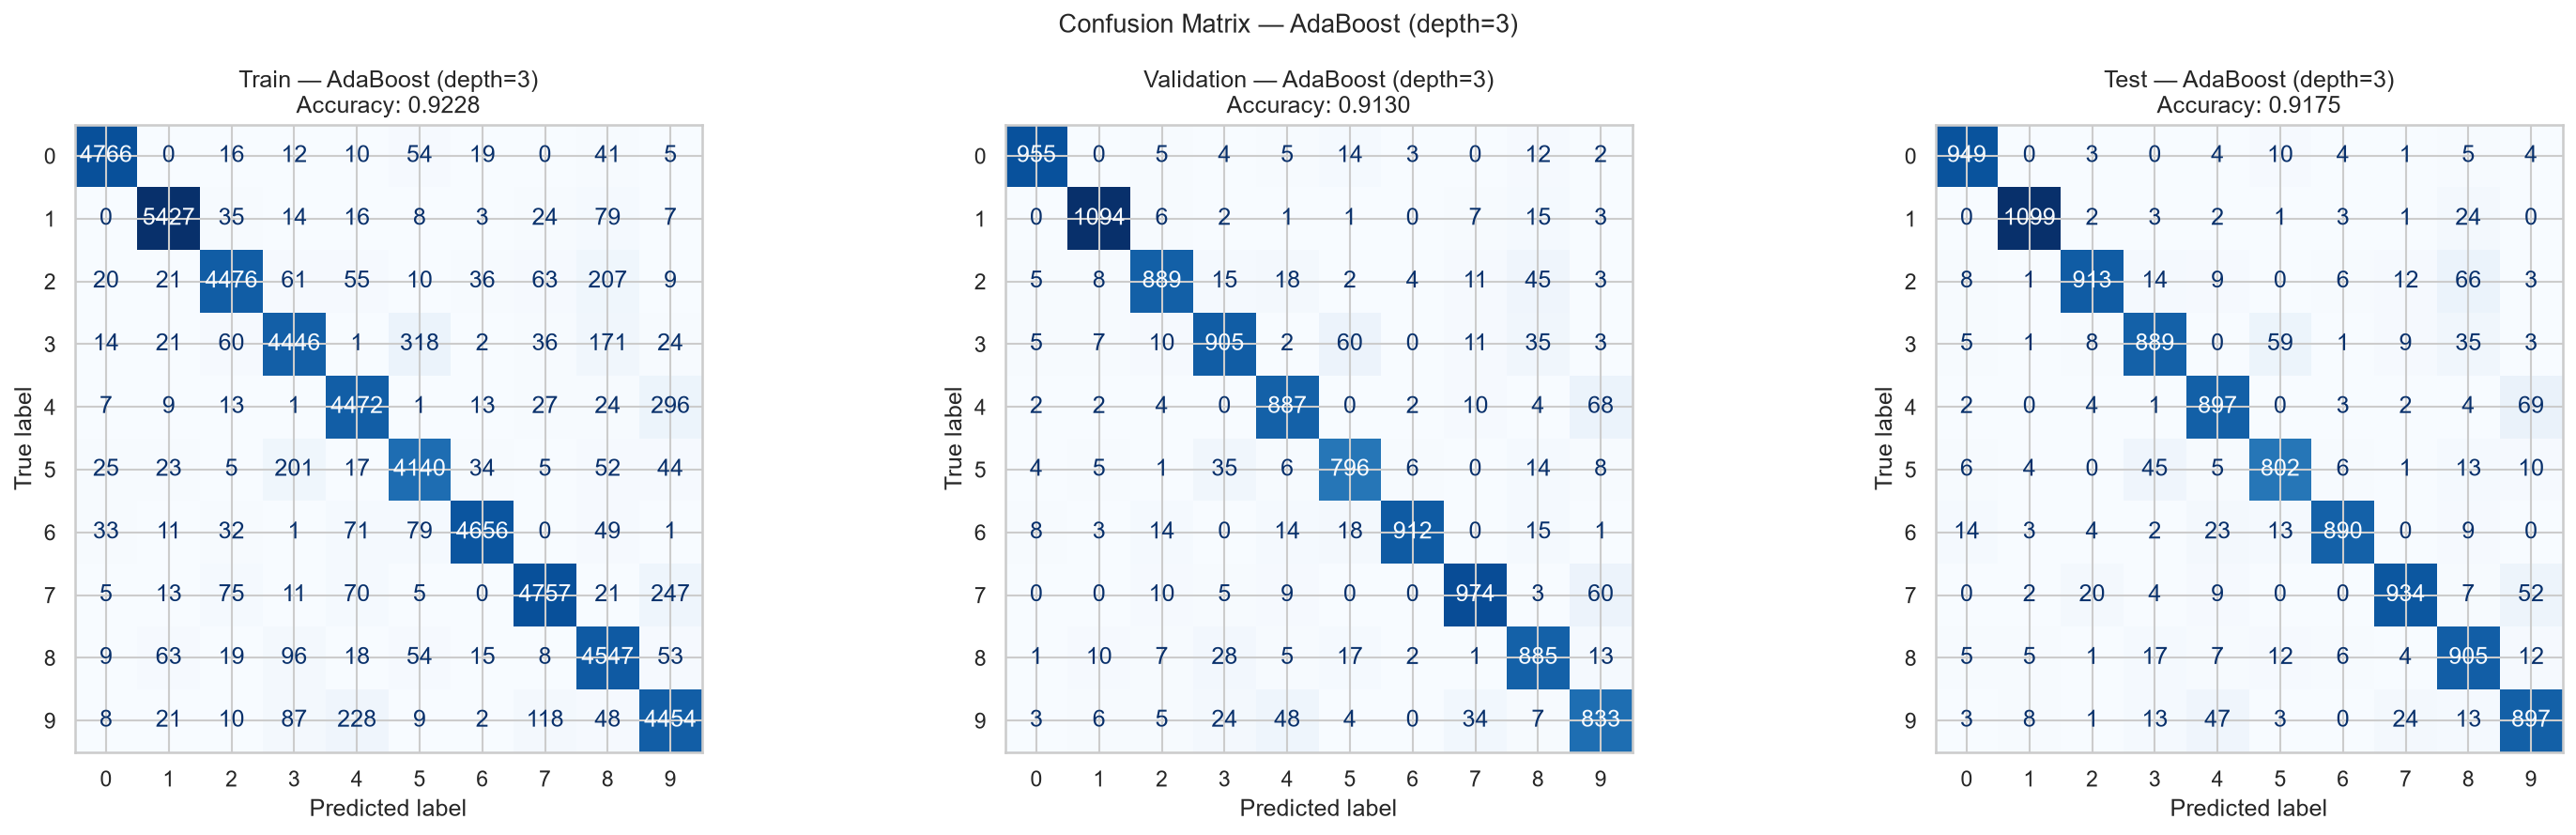
\includegraphics[width=0.58\textwidth]{4_02_confusion_matrix_best.png}
\caption{Ma trận nhầm lẫn trên tập Test -- AdaBoost với Decision Tree (depth $=3$).}
\end{figure}

\subsubsection{Nhận xét}
\begingroup\small
\begin{itemize}
  \item Trong bốn phương pháp được khảo sát, AdaBoost kết hợp Decision Tree (depth $=3$) đạt Accuracy cao nhất trên tập Validation (91,30\%), vượt Logistic Regression (84,48\%) và Decision Tree (depth $=1$) (77,28\%). Kết quả cho thấy việc tăng độ sâu của cây giúp mô hình học được các ranh giới phân loại phức tạp hơn. Trên tập Test, mô hình đạt Accuracy 91,75\% và Macro-F1 91,70\%, với chênh lệch Accuracy chỉ 0,45 điểm phần trăm so với Validation, cho thấy khả năng tổng quát hóa tương đối ổn định trên hai tập dữ liệu.
  \item Khảo sát siêu tham số cho thấy việc tăng \texttt{n\_estimators} giúp cải thiện Accuracy, đặc biệt từ 50 lên 100 vòng, nhưng mức cải thiện giảm dần khi số vòng boosting tăng cao. Đối với \texttt{learning\_rate}, giá trị quá nhỏ (như 0,01) khiến mô hình hội tụ chậm, trong khi khoảng 0,3--0,5 cho kết quả tốt nhất. Điểm đánh đổi thực nghiệm là việc tăng số vòng boosting cần được cân nhắc với chi phí huấn luyện tăng tuyến tính.
  \item Ma trận nhầm lẫn cho thấy phần lớn dự đoán tập trung trên đường chéo chính. Tương tự các mô hình khác, khó khăn với các chữ số có nét viết tương đồng. Điển hình là cặp 4 và 9 có 116 mẫu bị nhầm lẫn qua lại, cho thấy giới hạn của mô hình khi phân biệt những đặc trưng hình học tinh tế của hai chữ số này. Đây là nguyên nhân khiến AdaBoost chưa đạt độ chính xác cao hơn trên tập Test.
\end{itemize}
\endgroup

% -----------------------------------------------------------------------------
\section{So sánh tổng hợp và Đánh giá các tiêu chí}

\subsection{Bảng tổng hợp chỉ số metrics và thời gian chạy}
Bảng tổng hợp kết quả đo đạc trên cả 3 tập dữ liệu Train/Validation/Test của toàn bộ các phương pháp trong đề tài.

\begin{table}[H]
\centering\scriptsize
\caption{Kết quả thực nghiệm của năm mô hình đại diện (Train / Validation / Test).}
\renewcommand{\arraystretch}{1.05}
\begin{tabular}{llrrrrrr}
\toprule
\textbf{Mô hình}&\textbf{Tập}&\textbf{Acc}&\textbf{Prec}&\textbf{Rec}&\textbf{F1}&\textbf{Train (s)}&\textbf{Pred (s)}\\
\midrule
\multirow{3}{*}{Multinomial Naive Bayes}&Train (50000)&82.47&83.19&82.18&82.35&0.0541&1.4082\\
&Val (10000)&82.15&82.77&81.80&81.98&--&0.2857\\
&Test (10000)&83.56&84.24&83.25&83.41&--&0.2689\\\midrule
\multirow{3}{*}{Logistic Regression (OvR)}&Train (50000)&86.00&86.04&85.72&85.71&10.7028&0.1679\\
&Val (10000)&85.96&85.96&85.64&85.69&--&0.0284\\
&Test (10000)&86.84&86.87&86.58&86.55&--&0.0288\\\midrule
\multirow{3}{*}{AdaBoost (depth=3)}&Train (50000)&92.28&92.28&92.24&92.23&11019.2396&4.9749\\
&Val (10000)&91.30&91.28&91.22&91.22&--&2.7632\\
&Test (10000)&91.75&91.81&91.70&91.70&--&2.6681\\\midrule
\multirow{3}{*}{Multi-Layer Perceptron}&Train (50000)&100.00&100.00&100.00&100.00&33.5715&0.1142\\
&Val (10000)&97.88&97.85&97.87&97.86&--&0.0230\\
&Test (10000)&98.26&98.25&98.24&98.25&--&0.0216\\\midrule
\multirow{3}{*}{Convolutional Neural Net}&Train (50000)&99.65&99.65&99.65&99.65&51.6119&2.1970\\
&Val (10000)&98.58&98.57&98.57&98.57&--&0.4391\\
&Test (10000)&98.76&98.77&98.75&98.76&--&0.4285\\
\bottomrule
\end{tabular}
\end{table}

\subsection{Diễn giải kết quả và đánh giá cơ bản các mô hình}
\begin{enumerate}
  \item \textbf{Naive Bayes (83,56\%):} huấn luyện nhanh nhất (0,0541 s) nhưng bị giới hạn bởi giả định độc lập đặc trưng.
  \item \textbf{Logistic OvR (86,84\%):} suy luận nhanh nhất (0,0288 s/10.000 mẫu), cấu hình chuẩn hóa mới vượt Bayes 3,28 điểm \% nhờ tối ưu siêu tham số.
  \item \textbf{AdaBoost depth=3 (91,75\%):} cao hơn Logistic OvR 4,91 điểm \% và cao hơn Naive Bayes 8,19 điểm \%, đổi lại thời gian huấn luyện 11.019,24 s.
  \item \textbf{MLP (98,26\%):} đạt gần CNN và có thời gian dự đoán thấp nhất (0,0216 s/10.000 mẫu).
  \item \textbf{CNN (98,76\%):} tốt nhất về Accuracy và Macro-F1 nhờ khai thác cấu trúc không gian của ảnh.
\end{enumerate}

% Tệp tham chiếu đánh số lại cụm hình tổng hợp từ 13.
\setcounter{figure}{12}
\begin{figure}[H]
    \centering
    \begin{subfigure}[b]{0.98\textwidth}
        \centering
        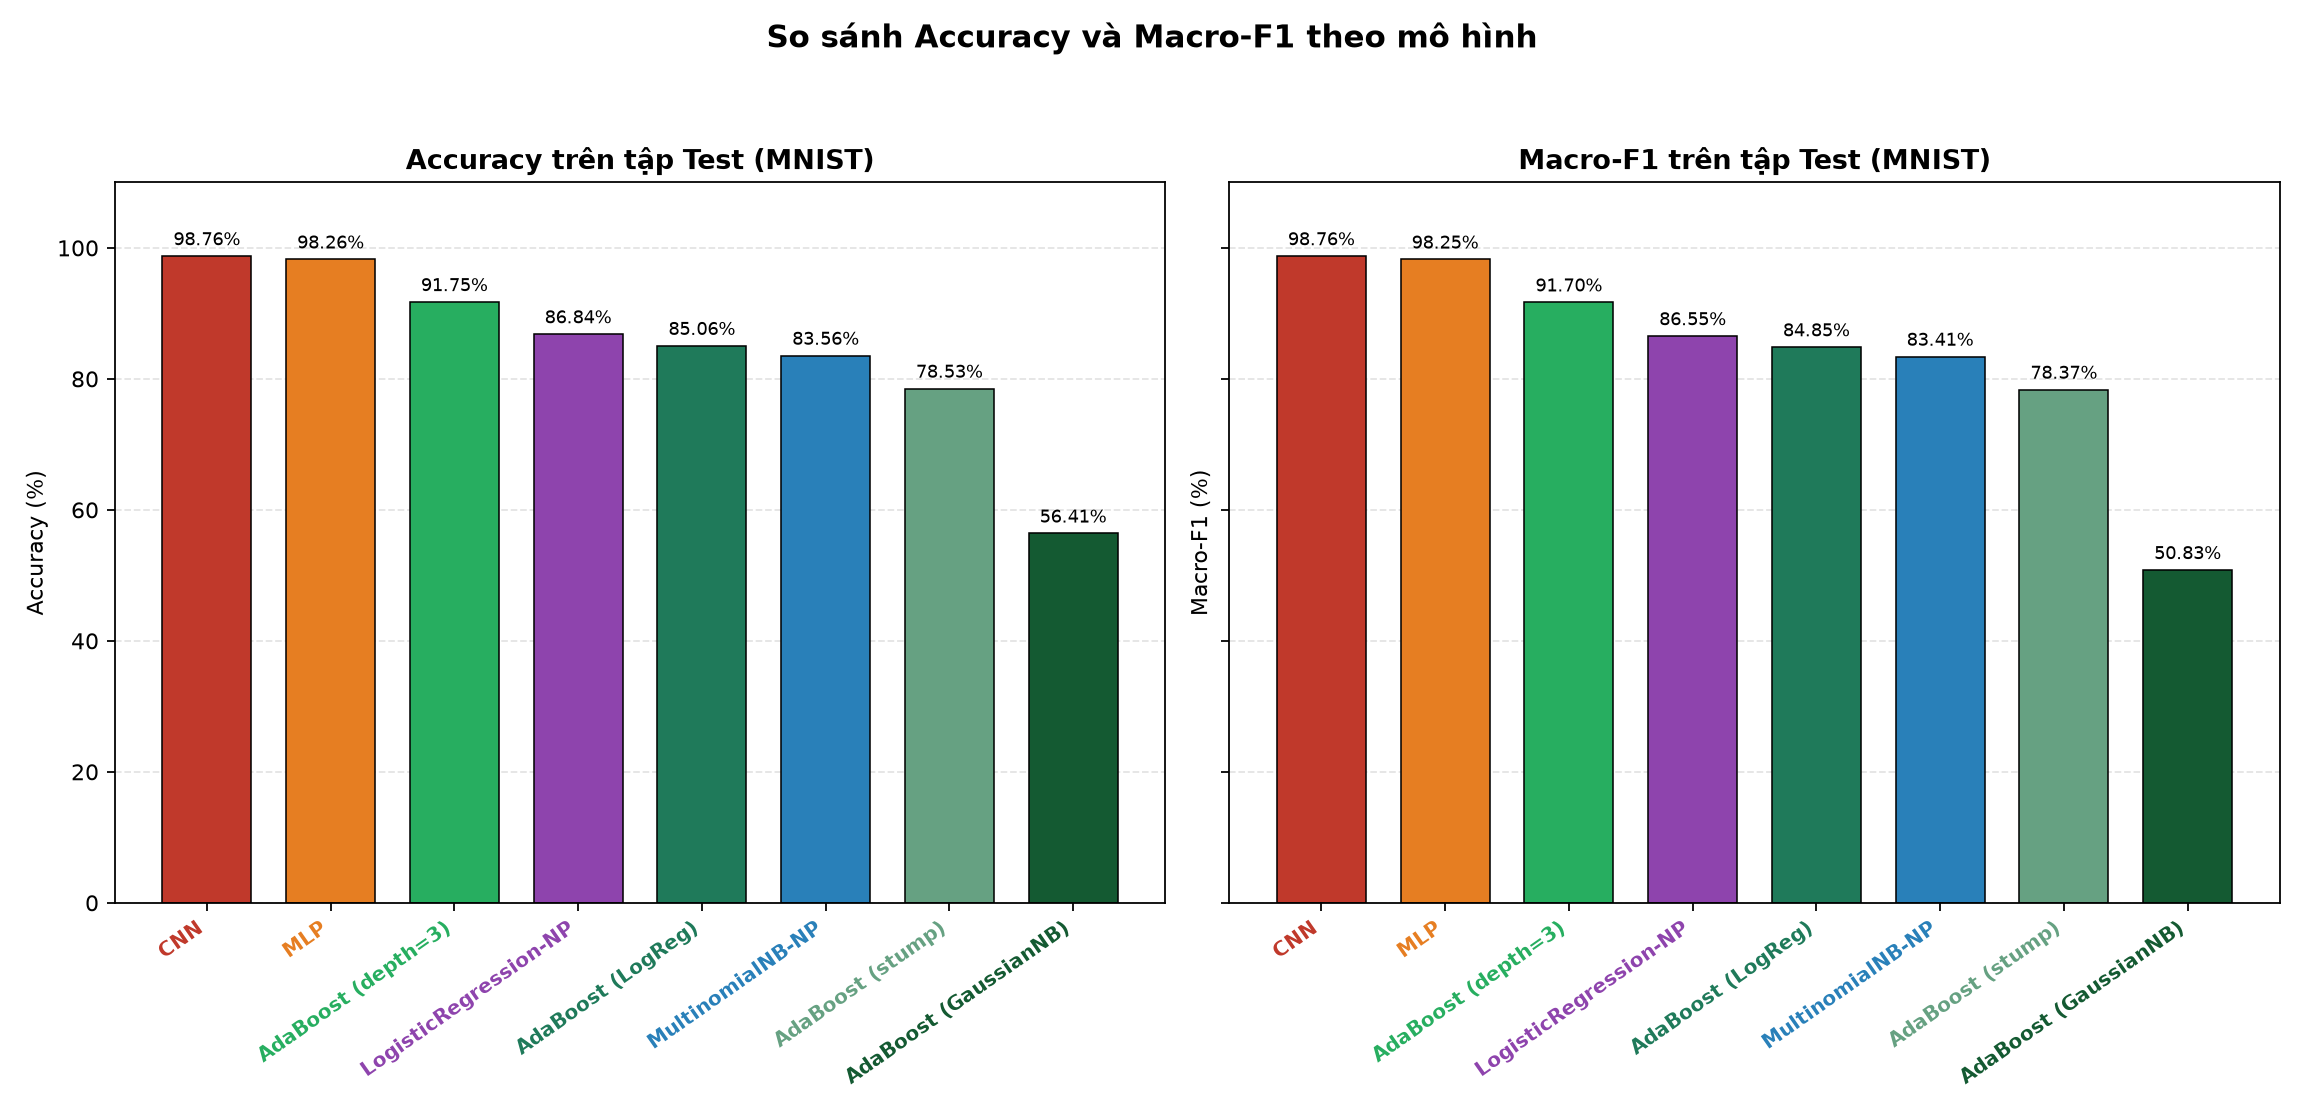
\includegraphics[width=\linewidth]{Comp_01_accuracy_f1_comparison.png}
        \caption{Accuracy và Macro-F1 của 8 cấu hình.}
    \end{subfigure}
\end{figure}


\vspace{0.3cm}
\setcounter{figure}{12}
\begin{figure}[H]
CNN đạt hiệu năng tốt nhất (Accuracy: 98,77\%, Macro-F1: 98,77\%), nhỉnh hơn 0,51\% so với MLP (98,26\% và 98,25\%). Trong nhóm học máy truyền thống, AdaBoost (depth=3) cao nhất (91,75\%), theo sau là Logistic Regression (86,84\%). Các mô hình còn lại như MultinomialNB, AdaBoost (stump/LogReg/GaussianNB) cho kết quả từ 56,41\% đến 85,06\%.
\vspace{0.5cm}
    \centering
\begin{subfigure}[b]{0.88\textwidth}
    \centering
    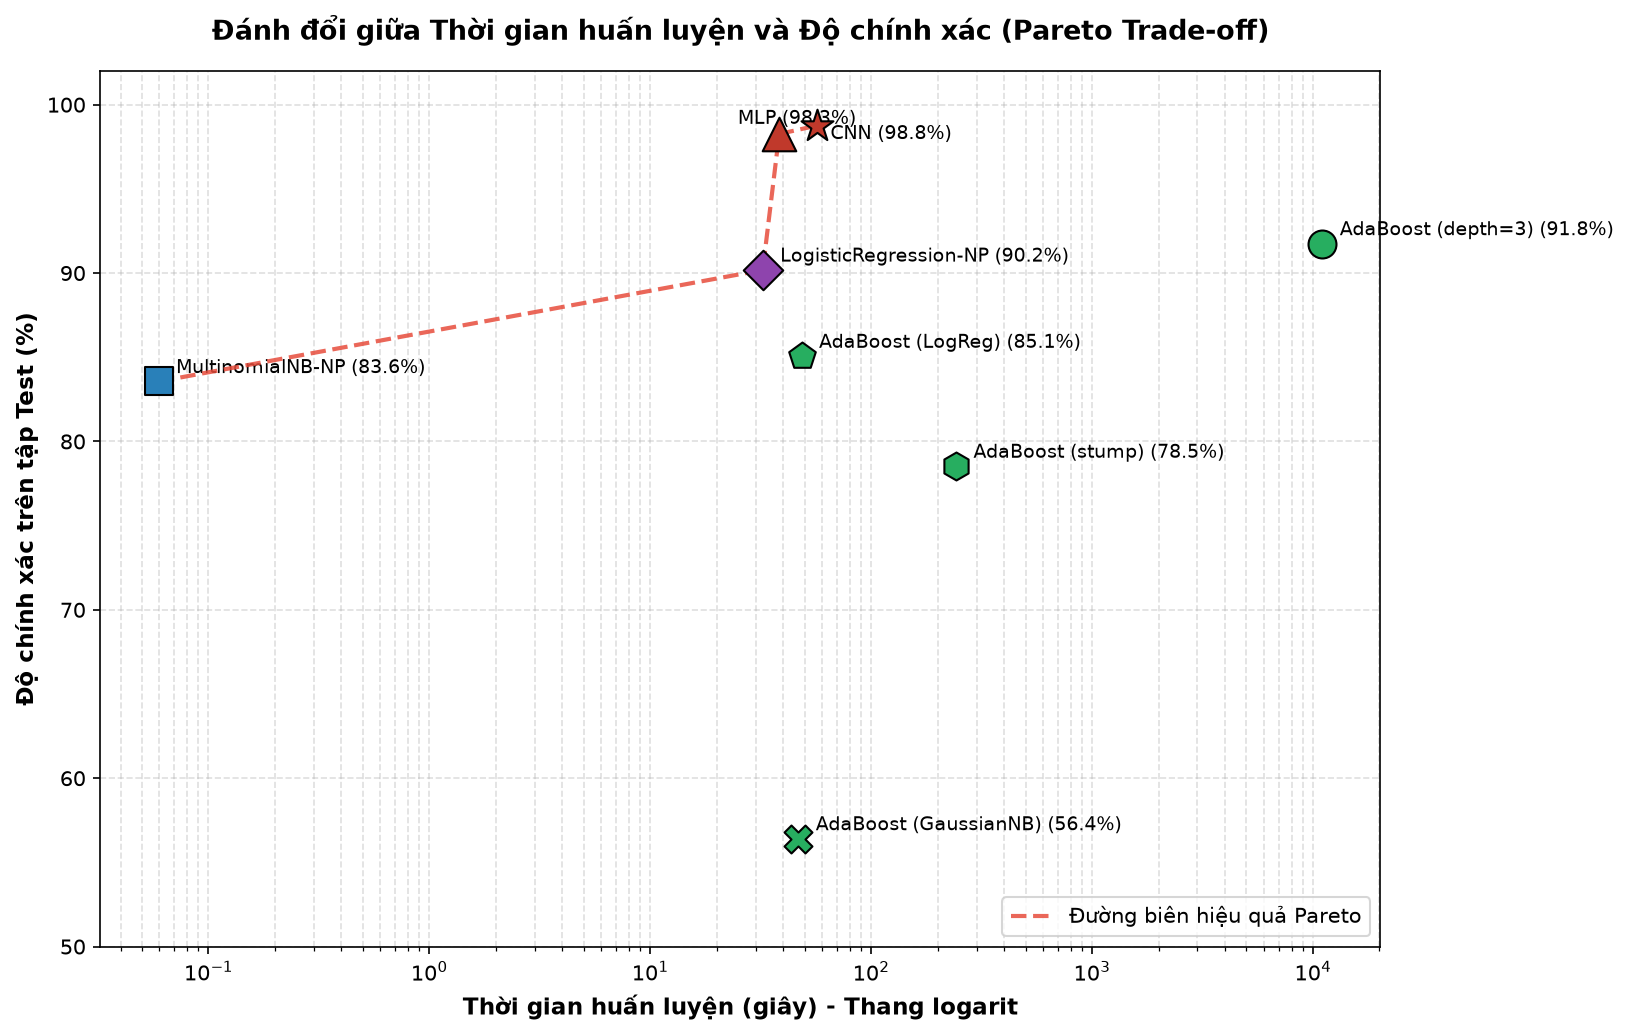
\includegraphics[width=\linewidth]{Comp_02_time_vs_accuracy_pareto.png}
    \caption{Đánh đổi thời gian huấn luyện -- Accuracy.}
    \end{subfigure}
    \caption{So sánh định lượng và biên hiệu quả Pareto từ dữ liệu thực nghiệm.}
\end{figure}

MultinomialNB có tốc độ huấn luyện nhanh nhất (0,06 giây). CNN (~43,6 giây) và MLP (~30,3 giây) mất nhiều thời gian hơn nhưng đánh đổi bằng độ chính xác vượt trội. Ngược lại, AdaBoost (depth=3) mất tới ~3 giờ (11.019 giây) huấn luyện do cấu trúc tuần tự trên ảnh phẳng, nhưng hiệu năng vẫn thấp hơn CNN 7,02\% do không tận dụng được đặc trưng không gian của dữ liệu ảnh.



\subsection{Phân tích và đưa ra kết luận mô hình tối ưu}
\begin{figure}[H]
    \centering
    \vspace*{0.3cm}
    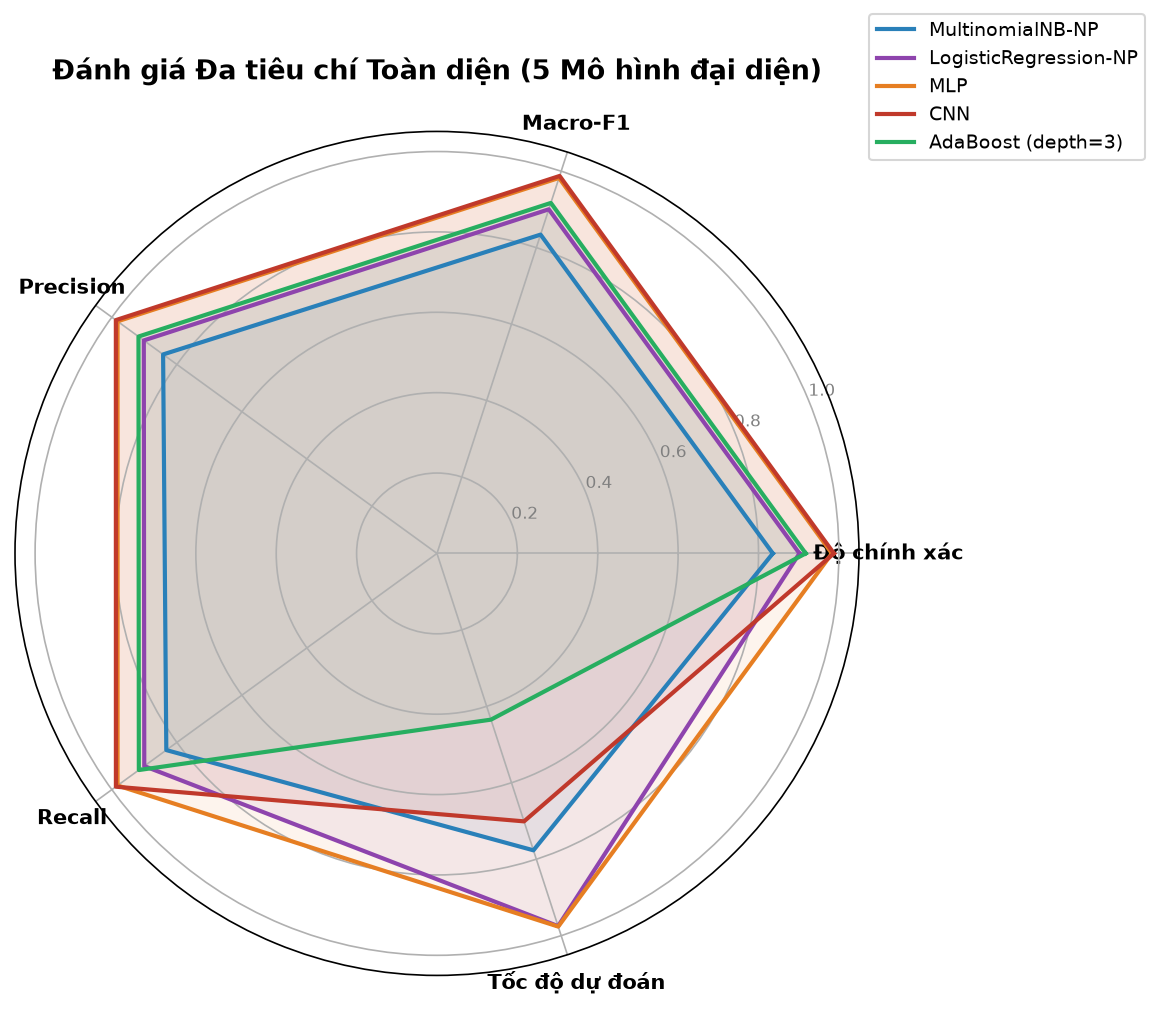
\includegraphics[width=0.8\textwidth]{Comp_03_radar_multi_criteria.png}
    \caption{Biểu đồ Radar đánh giá đa tiêu chí của năm mô hình.}
\end{figure}

Việc lựa chọn mô hình tối ưu phụ thuộc vào bài toán thực tế và sự đánh đổi giữa ba yếu tố cốt lõi: độ chính xác, tốc độ suy luận và chi phí huấn luyện. Dựa trên phân tích đa tiêu chí, kết quả thực nghiệm cho thấy các định hướng lựa chọn như sau:

\begin{itemize}
    \item \textbf{Ưu tiên độ chính xác tối đa:} CNN là lựa chọn hàng đầu nhờ khả năng khai thác cấu trúc ảnh 2D, đạt Accuracy 98,76\% với sai số chỉ 1,24\%. Tuy nhiên, mô hình này đòi hỏi thời gian huấn luyện lâu hơn và độ trễ suy luận (42,85 $\mu$s/mẫu) cao hơn so với các mô hình khác.
    
    \item \textbf{Cân bằng giữa hiệu năng và tốc độ (Lựa chọn tối ưu nhất):} MLP mang lại sự cân bằng xuất sắc. Dù Accuracy (98,26\%) thấp hơn CNN 0,50 điểm phần trăm, MLP sở hữu tốc độ suy diễn nhanh nhất (chỉ 2,16 $\mu$s/mẫu - nhanh hơn CNN gần 20 lần trên phép đo theo lô) và thời gian huấn luyện tương đối ngắn (33,57 giây).
    
    \item \textbf{Ưu tiên tốc độ huấn luyện và tài nguyên thấp:} Nhóm mô hình học máy truyền thống thể hiện rõ ưu thế này. MultinomialNB có tốc độ huấn luyện nhanh kỷ lục (0,054 giây) đạt Accuracy 83,56\%, cực kỳ phù hợp làm baseline hoặc cho các hệ thống cần cập nhật (train) liên tục. Logistic Regression (Accuracy 86,84\%) cũng là một giải pháp tốt với độ trễ thấp (2,88 $\mu$s/mẫu), cấu trúc nhỏ gọn (7.850 trọng số) và tính diễn giải cao.
    
    \item \textbf{Hạn chế của mô hình quần thể:} AdaBoost (depth=3) không khả thi cho bài toán này. Dù đạt độ chính xác khá (91,75\%), mô hình tiêu tốn lượng tài nguyên khổng lồ (hơn 3 giờ huấn luyện) và độ trễ suy luận rất cao (266,81 $\mu$s/mẫu).
    
    \item \textbf{Biên hiệu quả Pareto:} Khi xét đồng thời độ chính xác và thời gian huấn luyện, các mô hình MultinomialNB, Logistic Regression, MLP và CNN thiết lập nên một biên Pareto chuẩn mực (không có mô hình nào vượt trội hơn ở cả hai tiêu chí cùng lúc). Ngược lại, toàn bộ các cấu hình AdaBoost đều bị lấn át hoàn toàn, rơi ra khỏi đường biên này.
\end{itemize}

\vspace{0.3cm}
\noindent\textbf{Kết luận:} Việc triển khai mô hình vào thực tế sẽ tùy thuộc vào ràng buộc tài nguyên. CNN là giải pháp toàn diện nhất khi đặt độ chính xác làm trọng tâm. MLP là phương án tối ưu để triển khai ở môi trường cần suy luận (inference) nhanh nhưng vẫn đảm bảo độ chính xác cao. Cuối cùng, MultinomialNB và Logistic Regression đáp ứng hoàn hảo cho các tác vụ cần baseline siêu nhẹ, dễ diễn giải và có khả năng huấn luyện lại tức thì.
% -----------------------------------------------------------------------------
\section{Kết luận và Hướng phát triển}

\subsection{Kết luận}
Đồ án đã đạt được các kết quả nổi bật sau:
\begin{enumerate}
    \item Hoàn thiện pipeline tiền xử lý: xử lý 67 đặc trưng pixel có phương sai bằng 0 và ổn định tính toán số học bằng sigmoid phân nhánh, Log-Sum-Exp và Softmax dịch ngưỡng.
    \item Hiện thực hóa 5 mô hình từ cơ bản đến phức tạp: cài đặt thuần NumPy cho Multinomial Naive Bayes (83,56\%) và OvR Logistic Regression (82,53\%); triển khai học quần thể AdaBoost (91,75\%), và mạng học sâu MLP (98,26\%), CNN (98,76\%).
    \item Xây dựng hệ thống đánh giá thực nghiệm minh bạch và trực quan thông qua biểu đồ đánh đổi (Pareto), bản đồ nhiệt và ma trận nhầm lẫn.
\end{enumerate}

\subsection{Hạn chế và Hướng phát triển}
\begin{itemize}
    \item \textbf{Hạn chế:} Mô hình chưa được mở rộng thông qua các kỹ thuật tăng cường dữ liệu (Data Augmentation) như xoay, co giãn ảnh.
    \item \textbf{Hướng phát triển ngắn hạn:} Nghiên cứu phương pháp Ensemble (Soft-Voting) giữa CNN và AdaBoost; thử nghiệm kiến trúc ResNet và kỹ thuật lượng tử hóa (INT8) để triển khai trên vi điều khiển.
    \item \textbf{Hướng phát triển dài hạn - Hệ thống Web Demo Trực quan:} Xây dựng một nền tảng Web App nhận dạng chữ số viết tay toàn diện, cho phép tương tác trực tiếp với các mô hình:
    \begin{itemize}
        \item \textbf{Đa kênh đầu vào:} Cho phép vẽ trực tiếp trên canvas, tải ảnh lên hoặc chọn từ tập MNIST.
        \item \textbf{Phân tích đối chứng:} Dự đoán và so sánh chéo kết quả, xác suất, độ tin cậy của 5 mô hình trên cùng một mẫu dữ liệu.
        \item \textbf{Khám phá "Hộp đen" AI:} Trực quan hóa không gian 3D quá trình forward pass, quan sát feature map, kernel CNN và hoạt động của từng neuron từ dữ liệu thực tế.
        \item \textbf{Huấn luyện tương tác:} Cho phép người dùng tùy chỉnh tham số (epoch, learning rate, số mẫu), huấn luyện lại mô hình trực tiếp trên trình duyệt và xuất báo cáo (JSON trace).
    \end{itemize}
    Trải nghiệm hệ thống Web Demo tại:\\
    {\footnotesize\url{https://pattern-recognition-mnist-handwritten-digit-recognition.r2u-hcmus.workers.dev/}}
\end{itemize}

% -----------------------------------------------------------------------------
\section*{Phân công công việc nhóm và Khai báo sử dụng AI}
\addcontentsline{toc}{section}{Phân công công việc nhóm và Khai báo sử dụng AI}

\begin{table}[H]
\centering
\renewcommand{\arraystretch}{1.4} % Tăng khoảng cách giữa các dòng cho thoáng mắt
\small
\begin{tabularx}{\textwidth}{|l|c|X|c|}
\hline
\textbf{Thành viên} & \textbf{MSSV} & \multicolumn{1}{c|}{\textbf{Phần việc chi tiết đảm nhiệm}} & \textbf{Đóng góp} \\
\hline
\textbf{Trần Nguyên Hưng} & 24280048 & 
$\bullet$ Tiền xử lý dữ liệu MNIST và phân tích khám phá (EDA). \newline
$\bullet$ Cài đặt thuần (From Scratch): Multinomial Naive Bayes, OvR Logistic Regression. \newline
$\bullet$ Tinh chỉnh siêu tham số ($\alpha$, $\eta$), phân tích bản đồ trọng số \& ma trận nhầm lẫn. \newline
$\bullet$ Chịu trách nhiệm tổng hợp và soạn thảo báo cáo. & 
33.3\% \\
\hline
\textbf{Vương Thành Đạt} & 24280058 & 
$\bullet$ Cài đặt và khảo sát mạng nơ-ron đa tầng (MLP). \newline
$\bullet$ Khảo sát Inverted Dropout, tiêu biến gradient, khởi tạo trọng số (He/Xavier). \newline
$\bullet$ Thiết kế kiến trúc và huấn luyện mạng nơ-ron tích chập (CNN). \newline
$\bullet$ Thiết kế slide, chuẩn bị thuyết trình và hiệu chỉnh báo cáo. & 
33.3\% \\
\hline
\textbf{Phạm Phương Thảo} & 24280106 & 
$\bullet$ Nghiên cứu và cài đặt học quần thể (AdaBoost Ensemble). \newline
$\bullet$ Khảo sát tham số $N_{\text{estimators}}$, trích xuất độ quan trọng (Feature Importances). \newline
$\bullet$ Đánh giá, tổng hợp và so sánh toàn diện hiệu năng các mô hình. \newline
$\bullet$ Xây dựng và hoàn thiện hệ thống Web Demo trực quan. & 
33.4\% \\
\hline
\end{tabularx}
\end{table}

\noindent
\textbf{Khai báo sử dụng công cụ AI:} 

Trong quá trình thực hiện đồ án, nhóm có sử dụng các trợ lý AI (Gemini/ChatGPT) với vai trò công cụ hỗ trợ tiện ích nhằm tăng hiệu suất làm việc. Cụ thể, AI được dùng để tra cứu các cú pháp (NumPy, Matplotlib),tinh chỉnh định dạng văn bản LaTeX và hỗ trợ viết web deploy chương trình với mã nguồn của nhóm. 

Nhóm khẳng định toàn bộ flow thiết kế, mã nguồn hiện thực thuật toán lõi, cũng như quá trình phân tích đều được các thành viên tự nghiên cứu, bám bản chất bài dạy. Nhóm hoàn toàn làm chủ và chịu trách nhiệm về tính học thuật của đồ án.

% Thêm \usepackage{tcolorbox} ở đầu file .tex
\begin{tcolorbox}[colback=gray!8, colframe=black!75, title=\textbf{Mã nguồn và Tài nguyên Thực nghiệm (GitHub Repository)}, rounded corners, boxrule=0.8pt]
Toàn bộ mã nguồn cài đặt các thuật toán (From Scratch \& thư viện), pipeline tiền xử lý, kịch bản đánh giá cùng mã nguồn Web Demo được công bố mở tại:
\begin{center}
    \textbf{\url{https://github.com/gautrangtoidayyy/Pattern-Recognition}}
\end{center}
\end{tcolorbox}

\section*{Tài liệu tham khảo}
\addcontentsline{toc}{section}{Tài liệu tham khảo}
\begin{enumerate}[label={[\arabic*]}, noitemsep]
    \item Trương Phước Hưng, \textit{Slide Bài giảng Nhận dạng mẫu: Buổi 1-2 (Bayes Decision Theory), Buổi 3 (Linear Classifiers), Buổi 4 (MLP), Buổi 5 (Ensemble)}, Khoa CNTT, ĐH KHTN ĐHQG-HCM, 2026.
    \item Lê Phú Trường, \textit{Source code mẫu: Lab 2, Lab 3, Lab 4, Lab 5}.
    \item Christopher M. Bishop, \textit{Pattern Recognition and Machine Learning}, Springer, 2006. Mục 4.3.2 (Logistic Regression).
    \item Sergios Theodoridis, Konstantinos Koutroumbas, \textit{Pattern Recognition}, 4th Edition, Academic Press, 2008.
    \item Yann LeCun, Corinna Cortes, Christopher J.C. Burges, \textit{The MNIST Database of Handwritten Digits}, 1998.
\end{enumerate}


\end{document}
